%!TEX root = ../Thesis.tex
\chapter{Results}\label{cha:analysis}
This chapter contains the anomaly detection analysis performed on the data presented in \ref{sec:pelton_needles}. The goal is to investigate how well different methods detect anomalies when only being exposed to normal data during training. Three anomaly detection techniques are used, OC SVM, KDE and LSTM RNN. First, the different training sets and test cases are presented, then some prepossessing steps are introduced before the optimal hyperparameters of the different methods are presented. Finally, the performance of the different methods on the different cases is presented.

    \section{Training sets and test cases}
        Due to the aperiodic sampling of process signals, only the needle positions are sampled often enough to be included as features in the analysis. This means that the techniques for feature and dimensionality reduction presented in chapter \ref{cha:litterature} will not be used. The anomaly detection techniques are trained on three different training sets and evaluated on four test cases. The goal is to analyze how the methods evaluate the different cases when trained on different training sets. 
        
        \begin{table}[]
            \centering
            \begin{tabular}{ccccccc}
                \toprule
                \textbf{Set}    & \textbf{Plant}       & \textbf{Needle}   & \textbf{Train}  & \textbf{Validation}        & \textbf{T. samples}\\ \midrule
                1       & 1                    & 2,4        & 20170304-20170701 & 20170701-20170825 & 9449\\ 
                2       & 2                    & 2,4        & 20160422-20160506 & 20160506-20161001 & 12870\\ 
                3       & 2                    & 2,4        & 20160101-20160506 & 20160506-20161001 & 84263\\ \bottomrule
            \end{tabular}
            \caption{Table over the three different training sets}
            \label{tab:training_cases}
        \end{table}
        
        The three different training sets are presented in Table \ref{tab:training_cases}. Training set 1 is from Plant 1 turbine 2 after the reported incident when the needle operation is back to normal. There is no golden rule for the ratio between testing and validation, but according to \cite{Kohavi1995} somewhere around $1/3$ of the data is common to use for validation. Only seven months of data is available from Plant 1 turbine 2 after the needles are fixed. Therefore five months are used as training data and little under two months for validation. This resulted in a training set of 9449 samples. The validation data is used to ensure that the methods are not overfitting on the training data. Training set 2 and 3 are taken from Plant 2 turbine 2, which has no reported incidents and normal system operation over the entire sample period. Set 2 is similar to set 1 in size, set 3 is 10 times larger. This is done to evaluate if the performance of the anomaly detection techniques changes when exposed to more or less data during training. The same data is used for validation for both sets. The validation data is larger simply because there is more data available. Data from 2016 was picked because it represented all operational modes well. 
        
        \begin{table}[]
            \centering
            \begin{tabular}{ccccc}
                \toprule
                \textbf{Case}    & \textbf{Plant} & \textbf{Turbine}   & \textbf{Needle pair}   & \textbf{Data}               \\ \midrule
                1       & 1     & 2         & 2,4           & 20140101-20170304     \\ 
                2       & 2     & 2         & 2,4           & 20161001-20170401     \\ 
                3       & 1     & 1         & 2,4           & 20140801-20150201     \\ 
                4       & 1     & 2         & 1,3           & 20160601-20161101     \\ \bottomrule
            \end{tabular}
            \caption{Table over the four different test cases}
            \label{tab:test_cases}
        \end{table}
        
        Table \ref{tab:test_cases} shows the four test cases. The first case is all data from Plant 1 turbine 2 up until the incident, as the data after is used for training. As this is the needle pair with the recorded incident, it is interesting to see how the different methods evaluate the data, especially building up towards the incident. Case 2 is the artificial case introduced in \ref{subsec:arti} where an artificial error is added to normal data from plant 2. The artificial error is added from 20170201. Hence, all data from 2016 is normal plant data. The artificial case enables one to evaluate how early the methods detect anomalies when knowing exactly the start date of the system degradation. Case 3 and 4 are data surrounding the reported start failures introduced in \ref{subsec:start_failures}. The start-up failures will help evaluate how well the methods recognizes known abnormal patterns in the data. 
        
        Training and evaluating the methods on data from different plants and turbines enables one to evaluate cross plant performance. This is very interesting, if it can be shown that one can simply deploy a pre-trained anomaly detection system at new plants with little to no alteration, this will greatly reduce the cost of installing such systems. 
        
        
        
    \section{Prepossessing steps}
        The data needs to be preprocessed before it can be analyzed. First, all time steps where not both needles are sampled are removed. Secondly, \cite{Tarassenko2009} talks about the importance of removing steady-state samples from the dataset, to avoid biasing the data.  The needles are constantly changing during operation, hence the only steady state is when the plant is not operating. Steady state is removed by removing all samples where the process signal values are close to zero ($<2$) and unchanged since the last sample. Having a stationary time series is important. As \cite{Manuca1996} explains, many of the common techniques for analyzing time series assume that the given series is stationary. A stationary time series is said to be independent of time, and don't have any correlations with seasonality. As the no operation data is removed from this dataset, the data is seen as stationary. The next step is to scale the data. For OC SVM and KDE, the data is scaled to zero mean and unit variance, for the LSTM RNN the data is scaled within a range of [0,1]. This was found to yield the optimal behavior for the different algorithms. To enable cross testing between plants, the transformations are calculated on plant 1 turbine 2 needles [2,4] and used for all datasets. Finally, the data is checked for outliers using scatterplots, as having anomalies in the training data could damage the systems ability to detect anomalies. 
    
    \section{Hyperparameterization}
        The methods chosen for the anomaly detection have several different parameters or hyperparameters. To ensure that the methods perform optimally, it is necessary to search for the best combination of these parameters. To enable comparing the different cases analyzed, an optimal parameterization is found and used for all cases. The hyperparameter search is performed on the data sampled from plant 1 turbine 2 needle [2,4], after the reported incident. 
            \subsection{One class support vector machine}
                The OC SVM has two tunable parameters. These are $\gamma$ and $\nu$. There is, however, no good way to automatically find the optimal parameterization for unlabeled data. By default, one has to inspect the one class SVM performance for different hyperparameterizations manually. It is attempted to create a custom cost function for automatic hyperparameterization. The cost function builds upon the idea that a good separating hyperplane or decision boundary lay close to the samples. The OC SVM implementation in scikit-learn stores the signed distance from each sample to the separating hyperplane. The distance can be used to evaluate the shape of the decision boundary. The proposed cost function is seen in equation \ref{eq:svm_cost} where $\bm{x}$ is the vector with the signed distances for each sample to the separating hyperplane. Several setups for a cost function were tried. The chosen performed well for the cases studied in this thesis. One cannot guarantee that it will perform adequately for different cases.  
                
                \begin{align}
                    \score = 1 - \abs(\std(\bm{x})) - \abs(\mean(\bm{x})) -\frac{\outliers}{\inliers}100
                    \label{eq:svm_cost}
                \end{align}
            
                As explained in theory, $\nu$ is the upper boundary for the fraction of outliers. Since the data is assumed to be outlier free, it is natural to pick values for $\nu$ that lie around $\frac{1}{N}$ where $N$ is the number of samples. $\gamma$ is a measure of the complexity of the decision boundary and is therefore chosen to span a wide range of values. A grid search is performed over the values seen in the list below. 
                \begin{itemize}
                    \item $\gamma =  [0.01,0.05,0.1,0.2,0.4,0.8,1,2,4,8,16]$
                    \item $\nu = [\frac{1}{25N}, \frac{1}{10N},\frac{1}{5N},\frac{1}{2N},\frac{1}{N},\frac{2}{N},\frac{5}{N},\frac{10}{N}]$
                    \label{list:svm_grid}
                \end{itemize}
                
                \begin{table}[h]
                    \centering
                    \begin{tabular}{ccc}
                        \toprule
                         \textbf{Score}  &   $\bm \gamma$    & $\bm \nu$         \\ \midrule
                         0.975  &   $0.05$      & $\frac{1}{N}$ \\ 
                         0.970  &   $0.1$      & $\frac{1}{2N}$ \\ 
                         0.961  &   $0.1$      & $\frac{1}{N}$ \\ 
                         0.960  &   $0.05$      & $\frac{2}{N}$ \\ 
                         0.957  &   $0.2$       & $\frac{1}{N}$ \\ 
                         -44.437  &   $8$      & $\frac{1}{10N}$ \\ 
                         -51.780  &   $8$      & $\frac{1}{25N}$ \\ 
                         -57.461  &   $0.1$      & $\frac{1}{25N}$ \\
                         -71.082  &   $16$      & $\frac{1}{10N}$ \\ 
                         -506.263  &   $16$      & $\frac{1}{25N}$ \\ \bottomrule
                         
                    \end{tabular}
                    \caption{Table showing the five best and five worst scores for the gridsearch after optimal hyperparameters for the one class SVM. $N = $ number of samples.}
                    \label{tab:svm_gridsearch}
                \end{table}
                
                Table \ref{tab:svm_gridsearch} shows the score for the five best and five worst hyperparameterizations. It can be seen that a too low $\nu$ or a too large $\gamma$ yields the worst performance. Figure \ref{fig:svm_grid_best} shows the decision boundary for the classifier that scored the best with regards of the cost function defined in equation \ref{eq:svm_cost}. All samples located inside the red boundary line, are classified as normal, and points outside as anomalies. The boundary covers all samples with a reasonable distance from the samples. As can be seen, most of the support vectors are located at the upper and lower range of the samples, showing the importance of having training data that span the full operating range of the machinery. A couple of samples in the mid area are also picked as support vectors. This gives a relatively close, but smooth boundary. The boundary for the worst parameterization is seen in Figure \ref{fig:svm_grid_wors}, it is easily verified that the boundary is to complex, due to a large $\gamma$ and a very small $\nu$. The decision boundaries for the remaining classifiers seen in table \ref{tab:svm_gridsearch}, are found in appendix \ref{apendix:svm_grid}. It is verified that all of the high scoring classifiers have a similar shape of the decision boundary. Note that the plots are produced using the scaled data. 
                
                \begin{figure}
                        \centering
                        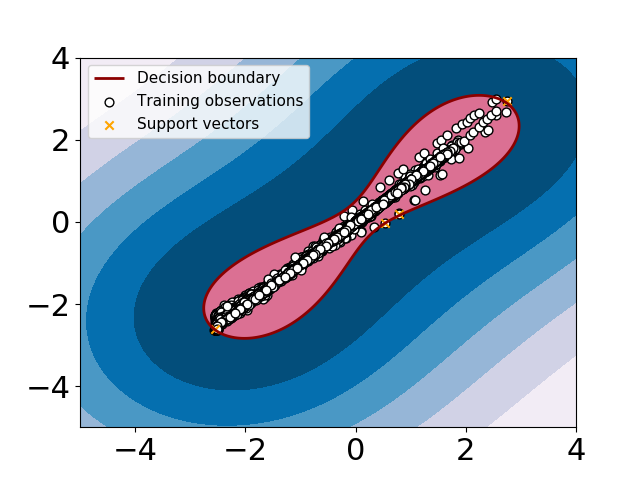
\includegraphics[width=0.7\textwidth]{report/figures/analysis/gridsearch/Novelty detection, 1, training, gamma = 0.05 nu = 1.0583130489998942e-05.png}
                        \caption{Decision boundary for the best scoring classifier. All observations inside the red boundary are classified as normal, all observations outside as anomalies. The support vectors are seen in orange crosses. The color outside the boundary indicates the distance to the separating hyperplane.}
                        \label{fig:svm_grid_best}
                        
                \end{figure}
                
                \begin{figure}
                        \centering
                        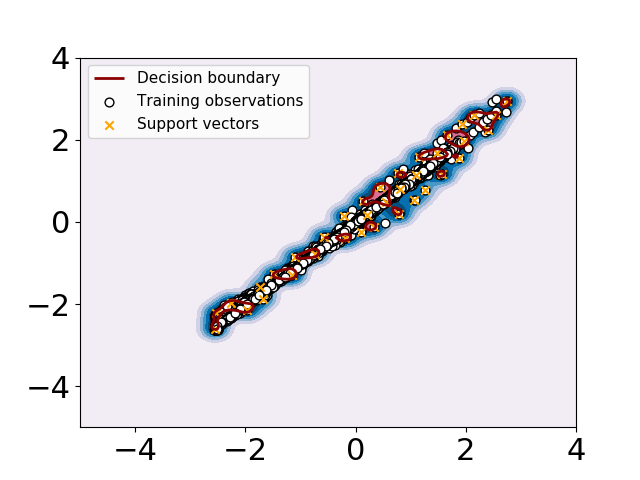
\includegraphics[width=0.7\textwidth]{report/figures/analysis/gridsearch/Novelty detection, -1 training, gamma = 16 nu = 4.233252195999577e-06.png}
                        \caption{Decision boundary for the worst classifier. How to interpret the figure is found in Figure \ref{fig:svm_grid_best}}
                        \label{fig:svm_grid_wors}
                \end{figure}
    
                
                
            \subsection{Kernel density estimation}
                The optimal hyperparameters for KDE were found using the built-in grid search method in scikit-learn. The different parameterizations are scored based on how well they replicate the distribution of the original data. As with OC SVM, KDE only has two parameters, bandwidth and kernel type. The bandwidth serves as a smoothing parameter, the higher the bandwidth, the smoother the density estimation will become. The KDE grid search was performed over a bandwidth from $[0,1]$ at $0.1$ steps, and with Gaussian, Tophat, Epanechnikov, Exponential, Linear and Cosine as kernels. The optimal parameter combination was found to be the Gaussian kernel with $0.1$ as bandwidth. 
                
                
            \subsection{Long short term memory recurrent neural network}
                A custom grid search for the optimal hyperparameterization for the LSTM network was created. As the network is trained to recreate the input, the Euclidean norm of the difference between predicted and real value is used to score the performance of the network. The models were trained on a training set and tested on a validation set. The different parameters are shown in the list below.  
                \begin{itemize}
                    \item Epochs $= 100$
                    \item Batch size $=[8,32,128,1024]$
                    \item Neurons $= [2,4,8,16,32,64,128,256]$
                    \item Layers $= [1]$
                \end{itemize}
                A preliminary search found that increasing the layer depth introduced overfitting, and therefore only one layer was included in the grid search. The network consists of an LSTM layer with the number of neurons found in the grid search. In addition, there is a dense linear layer that recreates the input. The shape of the input is as required by Keras, transformed into a 3 dimensional tensor with dimension [num\_samples,num\_features,1]. Table \ref{tab:lstm_gri} shows the score for the five best and five worst parameter combinations. The grid search is performed with a maximum number of epochs set to $300$. Early stopping is used to avoid overfitting, and the optimal number of epochs for each parameterization is seen in the Table \ref{tab:lstm_gri}. Figure \ref{fig:lstm_grid_error_best} and \ref{fig:lstm_grid_error_worst} shows the training history plots for the best and worst configuration of the LSTM. As can be seen, the worst configuration is stopped after five epochs due to an increasing error in the test prediction. This is typical for models with high variance, which are prone to model random noise in the training set. Looking into the parameters for this configuration one can see that the batch size is very small, meaning that the network weights are updated after only being exposed to a small number of samples, this seems to cause overfitting. The best configuration is not stopped before it reaches 134 epochs, and as can be seen, it performs equally on both training and test data. The history plots for the eight other configurations can be found in appendix \ref{appendix:lstm_grid}. 
                
                
                % As can be seen the network performs best with one layer and a large number of neurons, the most important parameter seems to be the batch size, where smaller batch sizes outperform larger. Figure \ref{fig:lstm_grid_error_best} shows the model error for the optimal LSTM structure. As can be seen, the error gradually decrease towards 50 epochs,  but as it goes beyond, it can seem like there is a tendency to overfitting on the training data, as the test performance is changing, the training will, therefore, be stopped after 50 epochs. Figure \ref{fig:lstm_grid_worst} shows the model error for the worst parameterization. As can be seen, it performs a ten factor poorer than the best. Notice, however, that the model error is not converging, and hence the parametrization was tested by running for 300 epochs. Figure \ref{fig:lstm_worst_300} shows the result, as can be seen it converges, but still 
                
                \begin{table}[]
                    \centering
                    \begin{tabular}{ccccc}
                        \toprule
                        \textbf{Score}       & \textbf{Epochs}    & \textbf{Batch size}    & \textbf{Neurons}   & \textbf{layers}   \\ \midrule
                        $3.516e-03$     & $134$     & $256$          & $64$     & 1        \\ 
                        $3.521e-03$     & $288$     & $512$          & $16$      & 1        \\
                        $3.571e-03$     & $300$     & $1000$          & $64$      & 1    \\ 
                        $3.646e-03$     & $300$     & $1000$         & $128$      & 1   \\ 
                        $3.650e-03$     & $300$     & $256$         & $128$     & 1  \\ 
                        $0.026$         & $12$     & $16$          & $2$      & 1     \\
                        $0.026$         & $6$     & $16$        & $128$       & 1    \\ 
                        $0.026$         & $6$     & $16$        & $256$       & 1       \\ 
                        $0.031$         & $9$     & $8$          & $16$     & 1          \\
                        $0.046$         & $6$     & $8$          & $256$     & 1      \\ \bottomrule
                    \end{tabular}
                    \caption{Top five and bottom five scores after the grid search for optimal LSTM structure and parameters, the lower score the better the performance.}
                    \label{tab:lstm_gri}
                \end{table}
                
                \begin{figure}
                    \begin{minipage}[b]{0.49\linewidth}
                        \centering
                        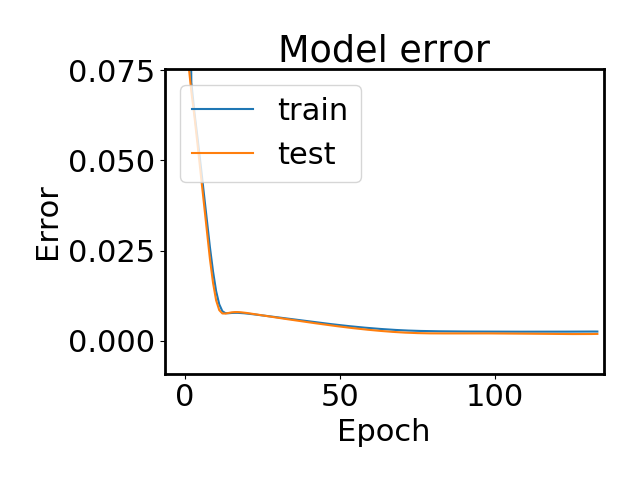
\includegraphics[width = \textwidth]{report/figures/analysis/lstm_gridsearch/best_lstm_error_zoomed.png}
                        \caption{Training history for the best LSTM configuration. Test and training prediction error is shown as a function of epochs.}
                        \label{fig:lstm_grid_error_best}
                    \end{minipage}
                    \hfill\vline\hfill
                    \begin{minipage}[b]{0.49\linewidth}
                        \centering
                        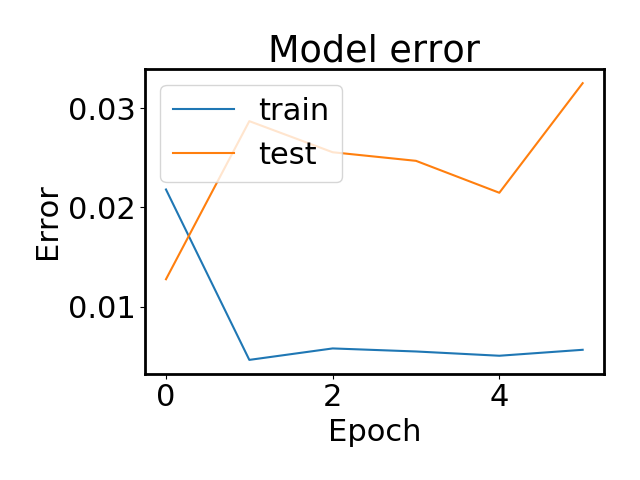
\includegraphics[width = \textwidth]{report/figures/analysis/lstm_gridsearch/worst_lstm_error_-1.png}
                        \caption{Training history for the worst LSTM configuration. Test and training prediction error is shown as a function of epochs.}
                        \label{fig:lstm_grid_error_worst}
                    \end{minipage}
                \end{figure}
        
    \section{Anomaly detection}
        Of the three methods used in the analysis, only OC SVM is a classifier. KDE and LSTM RNN gives an anomaly score. Hence they will be referenced as anomaly scorers. This means that to identify a sample as an anomaly, one needs to find a threshold for the anomaly score. This is not covered in the thesis.
        
    \subsection{Training set 1, test case 1 and 2}
        \begin{figure}
            \centering
            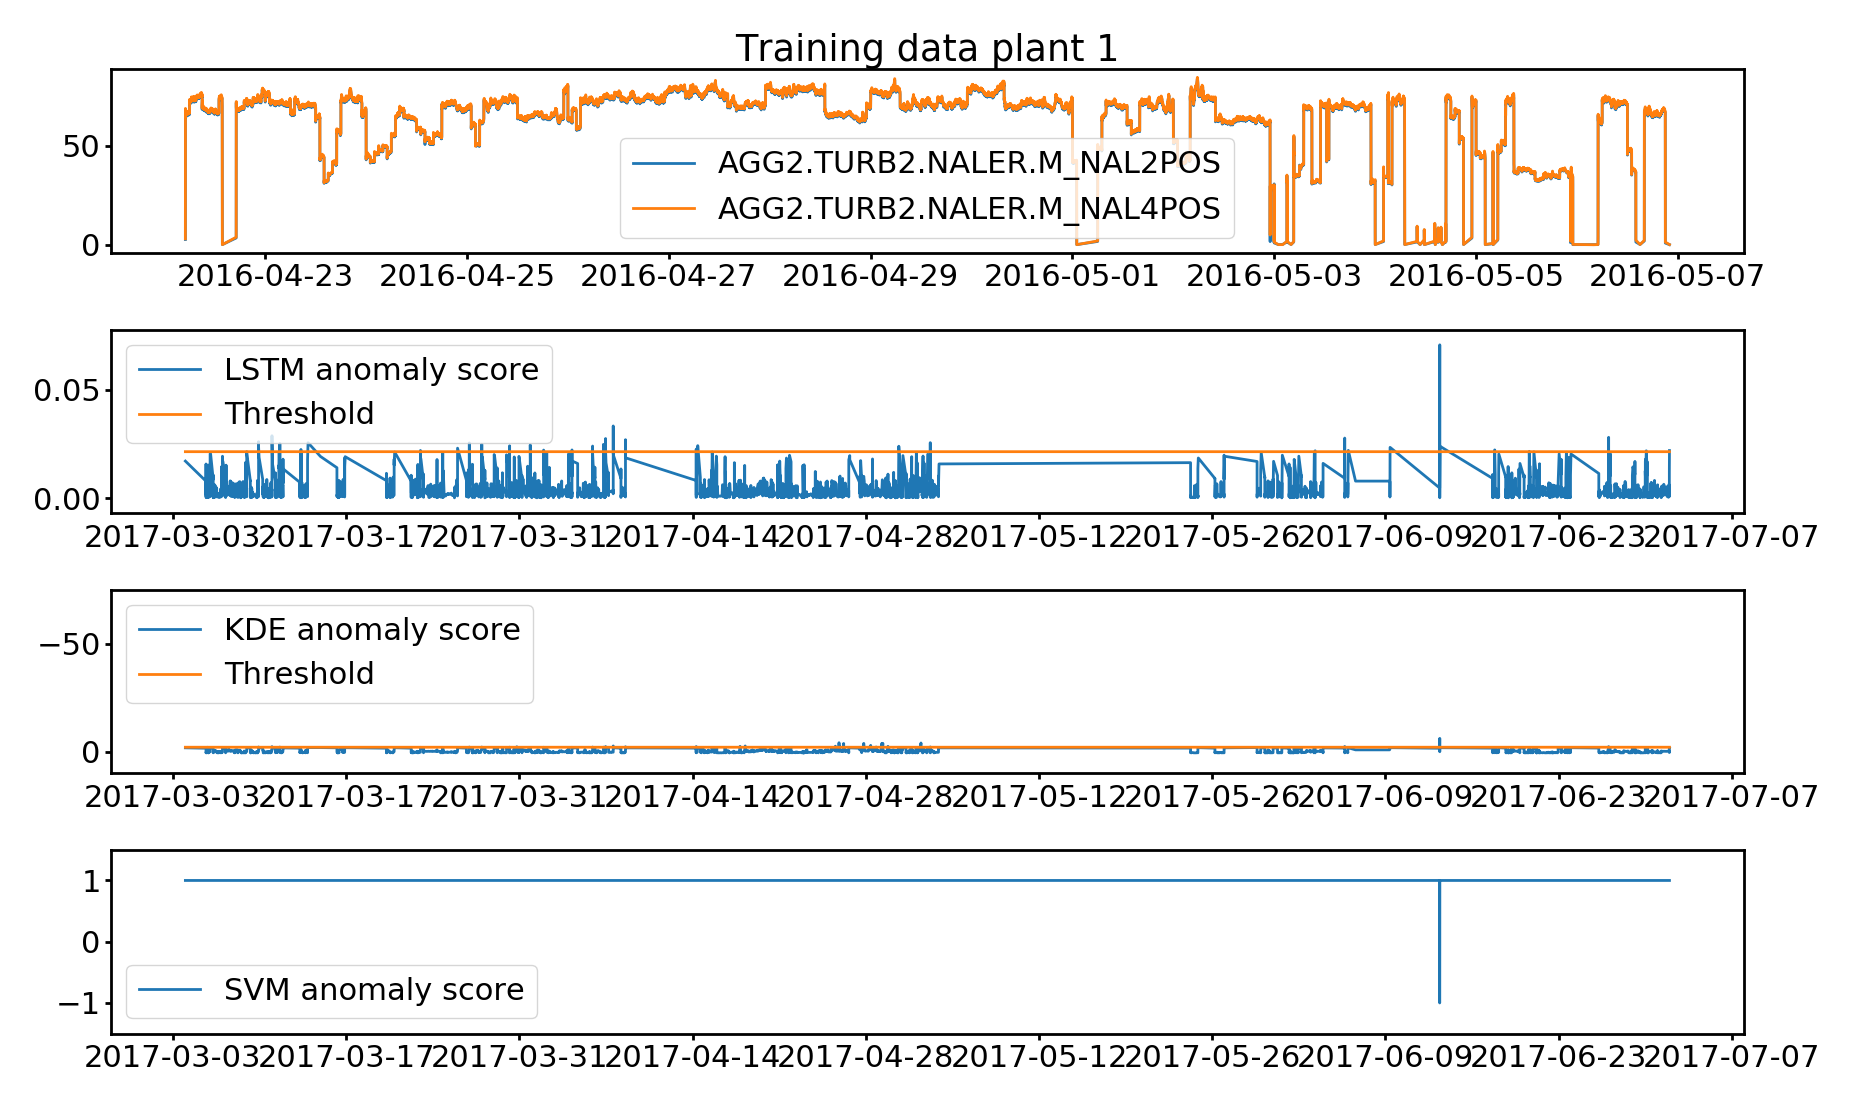
\includegraphics[width=\textwidth]{report/figures/analysis/plant1_training/training_data_anomaly.png}
            \caption{Training set 1 with the anomaly results for the different methods. The upper subplot shows the needle openings on top of each other. The second subplot shows how the LSTM anomaly scorer evaluates the data seen in the upper subplot, the higher the score, the more anomalous the data is. The third subplot shows the KDE scorer, the more negative the score is, the more anomalous the data is. The orange line in the two score plots indicates the 0.1\% most extreme scores. The last subplot shows how the OC SVM classifies the needle openings, normal = 1 and anomalous = -1.}
            \label{fig:anomaly_training_set1}
        \end{figure}
        Figure \ref{fig:anomaly_training_set1} shows training set 1, and how the different methods evaluate the training data. As can be seen, the anomaly scores for the KDE and LSTM anomaly scorers are similar in shape but different in magnitude. One data point is standing out from the rest for all three methods, but the anomaly score is still very close to the average. The same point is also evaluated as an anomaly for the OC SVM classifier.
        
        \begin{figure}
            \centering
            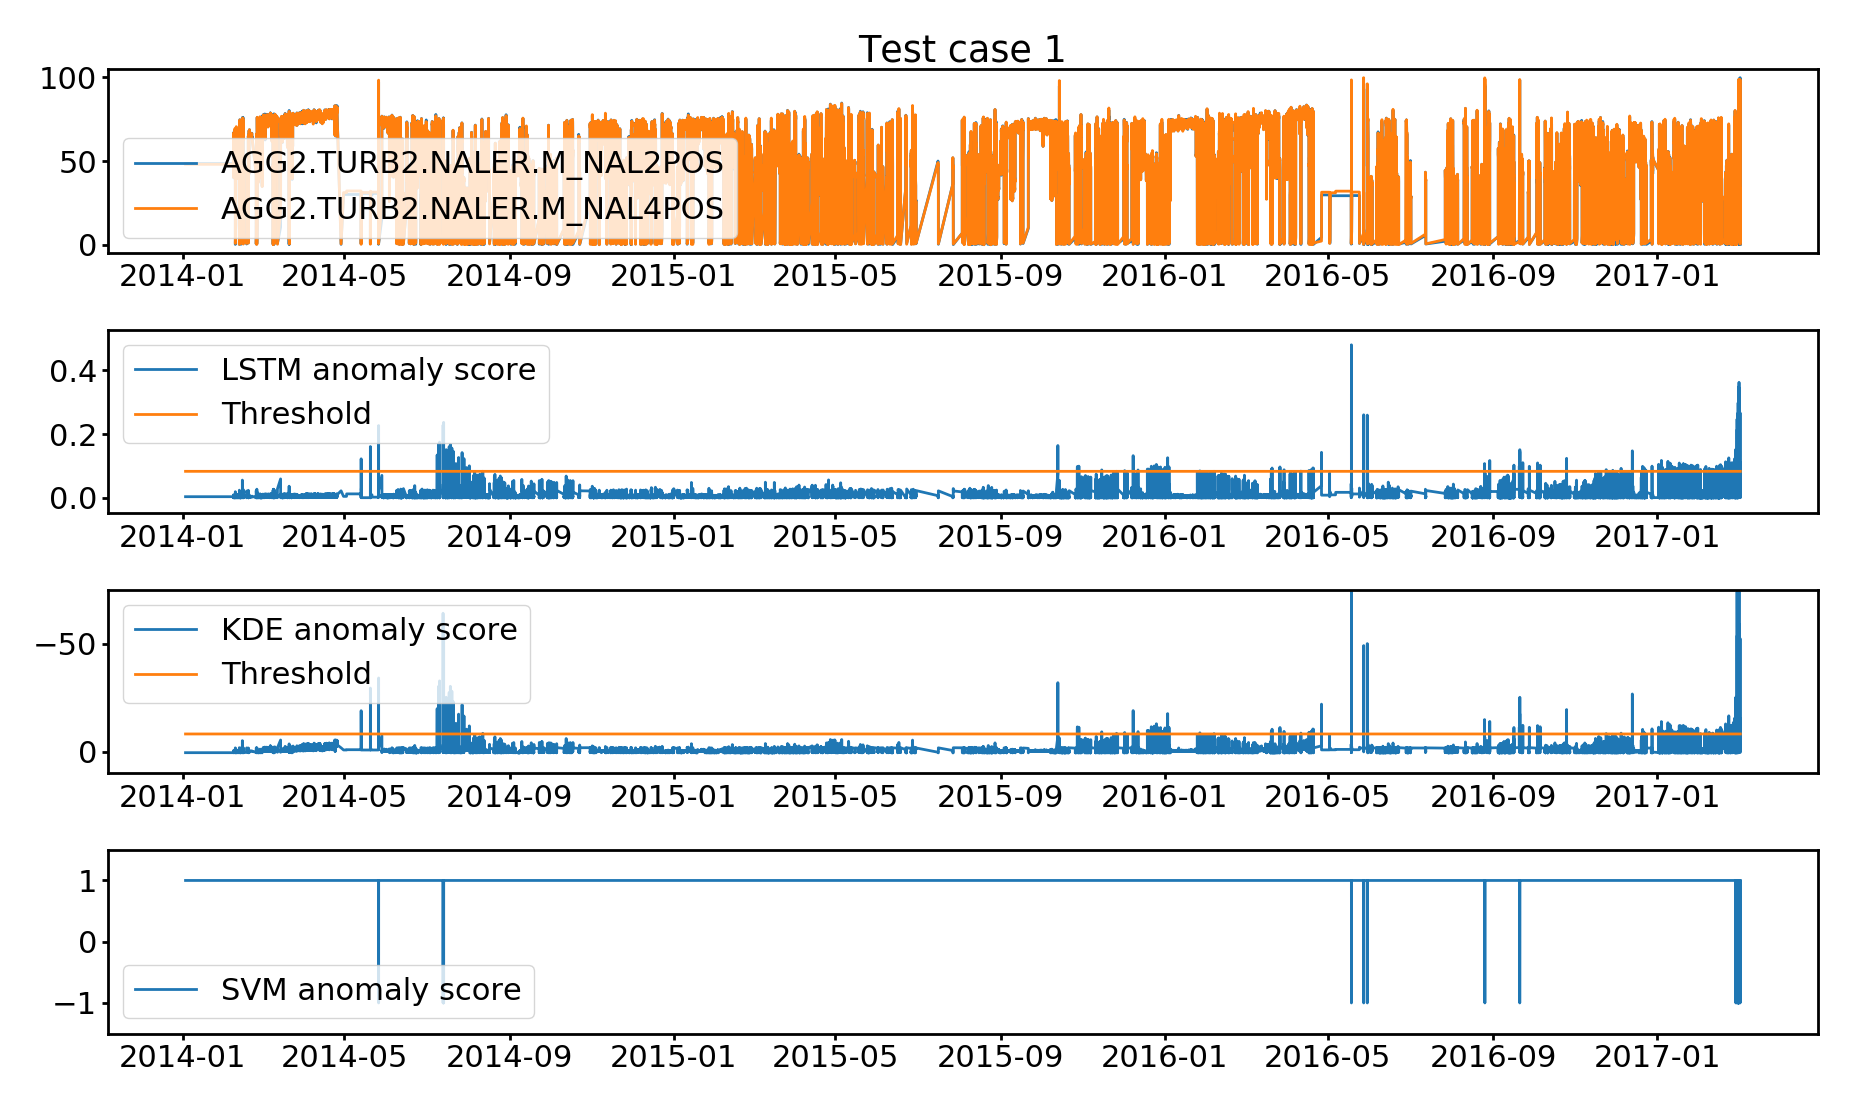
\includegraphics[width = \textwidth]{report/figures/analysis/plant1_training/production_data_anomaly.png}
            \caption{Anomaly results for the methods trained on training set 1 and evaluated on test case 1. For plot interpretation see Figure \ref{fig:anomaly_training_set1}.}
            \label{fig:anomaly_plant_1_train_production}
        \end{figure}
        Figure \ref{fig:anomaly_plant_1_train_production} shows the anomaly scores for the three different methods on test case 1. The top window shows the opening of the two needles. As can be seen, it is hard to spot any deviation between the two needles, even for the data from the reported incident at the end of the plot. For both the KDE and the LSTM anomaly scorers one can clearly see that the anomaly score of the data is increasing from September 2016. Several samples after January 2017 are located above the proposed threshold line. The anomaly score for both scorers is more than doubled from the score seen during the lowest periods. This shows that one can clearly identify that the scorers are detecting patterns in the data not seen during training, in the period leading up to the incident. This is verified by comparing the magnitude of the anomaly scores from figure \ref{fig:anomaly_training_set1} and \ref{fig:anomaly_plant_1_train_production}. Interestingly, there are also several samples spread out over the entire sampling period that is given a high anomaly score. This can be because the training set does not cover all modes of operation, operational problems or problems with data sampling. This trend is also seen in Figure \ref{fig:plant1_needle_error}. The power plant log did not report any operational issues except for the one in March 2017, but from the authors experience from the industry, it is not uncommon that not all maintenance work is logged. The OC SVM classifier is not able to detect a trend towards the incident. As can be seen, it only evaluates a few anomalies in the period up until the reported incident. There are also signs of abnormalities earlier in the production data as seen for the anomaly scorers. Interestingly, one can see that the samples evaluated as anomalies for the one class SVM are all among the highest scoring samples for the two anomaly scorers. 
        
        Table \ref{tab:trainining_plant1_stats} shows how the scorers evaluate the validation data compared to the data from test case 1. The plot for the anomaly scores of the validation set can be found in appendix \ref{appendix:training_case1}. In addition, boundary plots for the SVM classifier, KDE scorer and learning history plots for the LSTM scorer can be found there. As can be seen, there is a large difference between the minimum value for the validation and case data for the KDE scorer. There is also a difference between the mean values. This shows that the test case 1 data takes on patterns not seen in the validation data. The same trend is seen in the statistics for the LSTM scorer. In both cases, the most extreme observation between training and production is approximately 100 times larger.
        
        Figure \ref{fig:svm_1_outliers_stats_production} shows the number and percentage of anomalies for the OC SVM classifier for test case 1. As can be seen, the anomaly percentage of the anomalies detected in 2014 and 2016 is much lower than for the reported incident in 2017. This indicates that separating what could be false positives from true positives, could be solved by using an anomaly percentage threshold. 
        
        \begin{table}[]
            % \begin{minipage}[b]{0.48\linewidth}
            \centering
            \begin{tabular}{ccccc}
                \toprule
                            & \textbf{KDE validation}  & \textbf{KDE case 1}    & \textbf{LSTM validation} & \textbf{LSTM case 2}   \\ \midrule
                min         & -2.671    & -275.66           & 1.659e-04 & 9.716e-05         \\ 
                max         & 0.491     & 0.491             & 3.032e-2  & 0.400             \\ 
                mean        & -0.296    & -0.728            & 3.318e-03 & 6.200e-3          \\ \bottomrule
            \end{tabular}
            \caption{Table comparing the statistics for the KDE and LSTM anomaly detectors on the validation and case 1 data for training case 1}
            \label{tab:trainining_plant1_stats}
        \end{table}
        
        \begin{figure}
            \begin{minipage}[b]{0.49\linewidth}
                \centering
                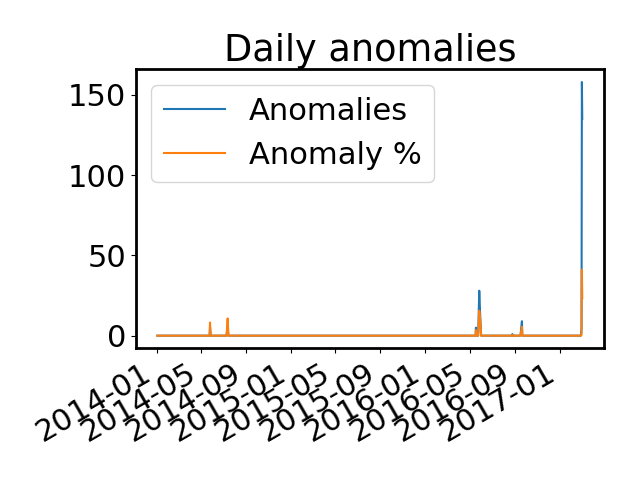
\includegraphics[width=\textwidth]{report/figures/analysis/plant1_training/daily_svm_outliers_production_small.png}
                \caption{Daily classified anomalies for the one class SVM classifier on production data}
                \label{fig:svm_1_outliers_stats_production}
            \end{minipage}
            \hfill\vline\hfill
            \begin{minipage}[b]{0.49\linewidth}
                \centering
                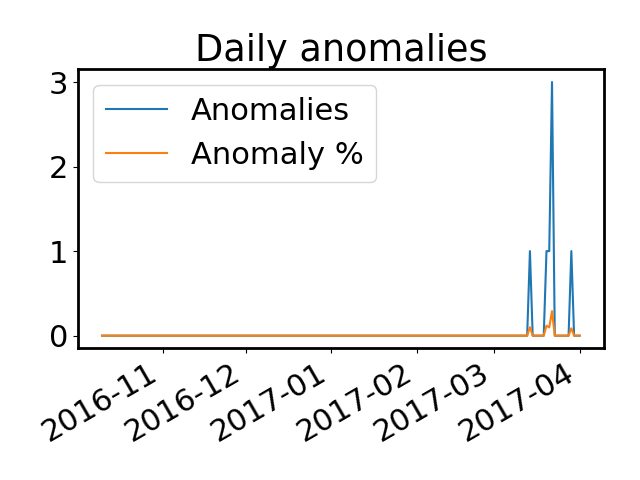
\includegraphics[width=\textwidth]{report/figures/analysis/plant1_training/daily_svm_outliers_artificial_small.png}
                \caption{Daily classified anomalies for the one class SVM classifier on artificial data}
                \label{fig:svm_1_outliers_stats_artificial}
            \end{minipage}
        \end{figure}
        
        Figure \ref{fig:anomaly_plant_1_train_artificial} shows the anomaly scores for test case 2. Note that test case 1 and 2 are from different plants. There is no sample data from January 2017, but since dates are used as indexes, January is still seen in the plot. The data from 2016 is normal data from plant 2, and the artificial error is gradually increasing from February to April in 2017. As can be seen, both the LSTM and KDE scorers have growing anomaly scores from mid-February. Towards March, the anomaly scores are significantly higher than for the normal data. Looking at figure \ref{fig:anomaly_plant_1_train_production} one can see that the anomaly score for the artificial error is of the same magnitude as the score for test case 1 in the months before the incidents. 
        
        The OC SVM classifier is not picking up the trend as fast as, but it clearly detects that something is wrong towards the end of the sample period. This can be verified by looking at \ref{fig:svm_1_outliers_stats_artificial}. Notice however how few samples that are classified as anomalous, and that the percentage is very low.      
        \begin{figure}
            \centering
            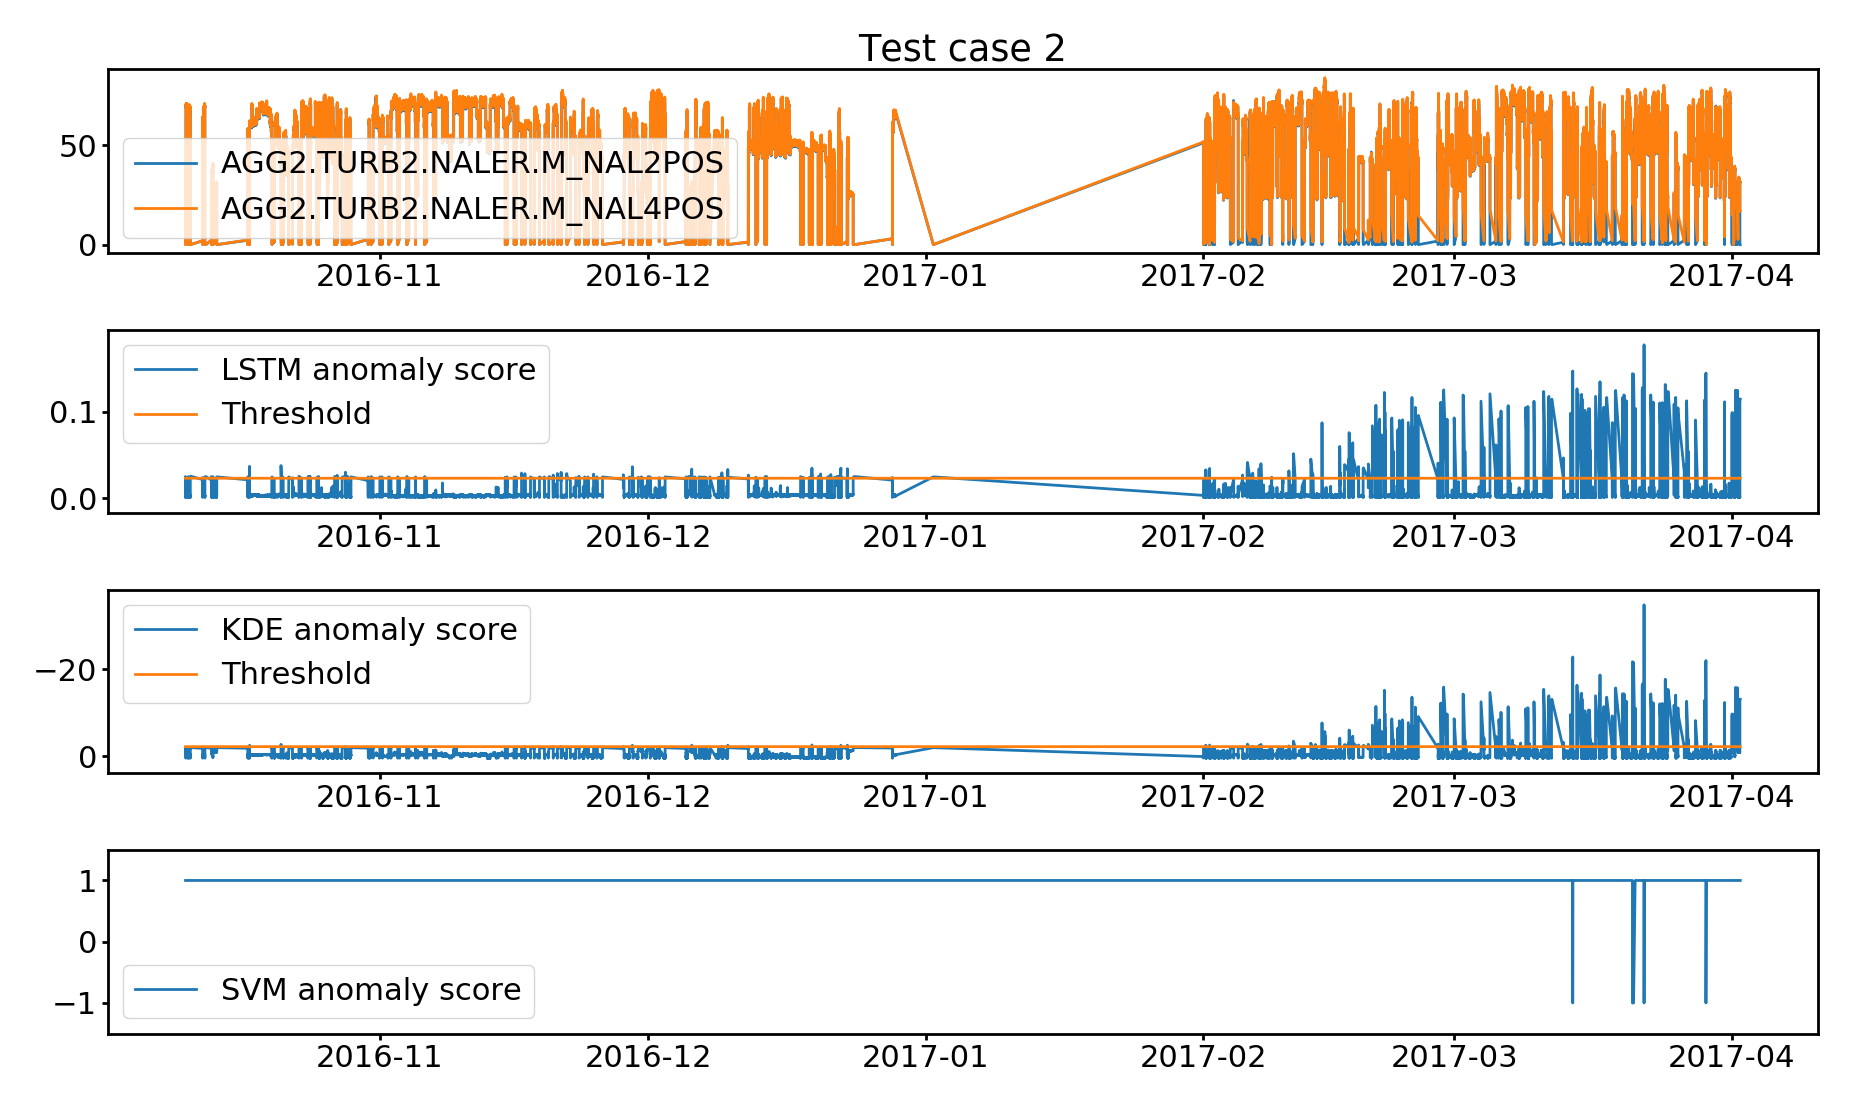
\includegraphics[width = \textwidth]{report/figures/analysis/plant1_training/artificial_data_anomaly.png}
            \caption{Anomaly results for the methods trained on training set 1 and evaluated on test case 2. For plot interpretation see Figure \ref{fig:anomaly_training_set1}.}
            \label{fig:anomaly_plant_1_train_artificial}
        \end{figure}
    
    \subsection{Training set 2, test case 1 and 2}
        \begin{figure}
            \centering
            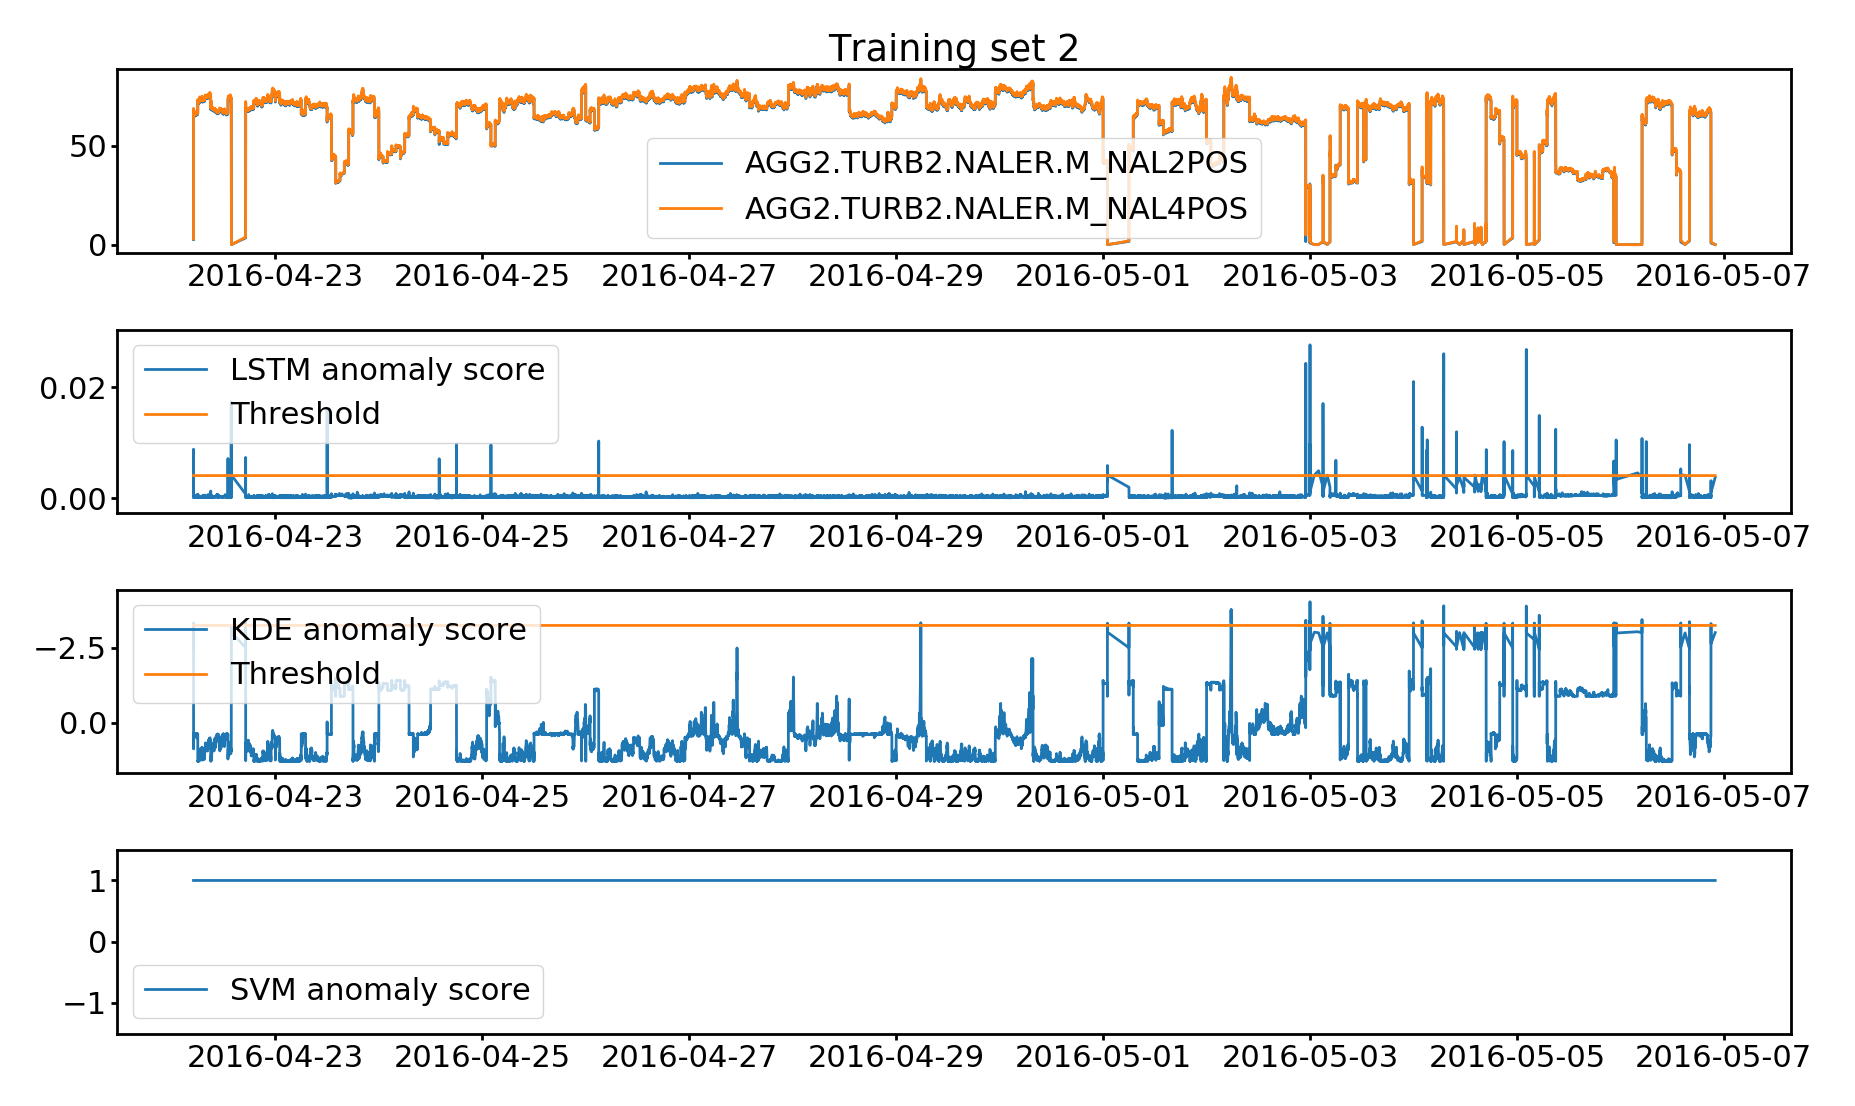
\includegraphics[width=\textwidth]{report/figures/analysis/plant2_train_short/training_data_anomaly.png}
            \caption{Anomaly results for the methods trained on training set 2 evaluated on training set 2. For plot interpretation see Figure \ref{fig:anomaly_training_set1}.}
            \label{fig:anomaly_training_set2}
        \end{figure}
        Figure \ref{fig:anomaly_training_set2} shows training set 2, and how the different methods evaluate the training data. As can be seen the anomaly scores for the KDE and LSTM anomaly scorers are not as similar in shape as was seen for training set 1. They are also reduced in magnitude. The OC SVM evaluates all data points as normal. 
    
        \begin{figure}[h!]
            \centering
            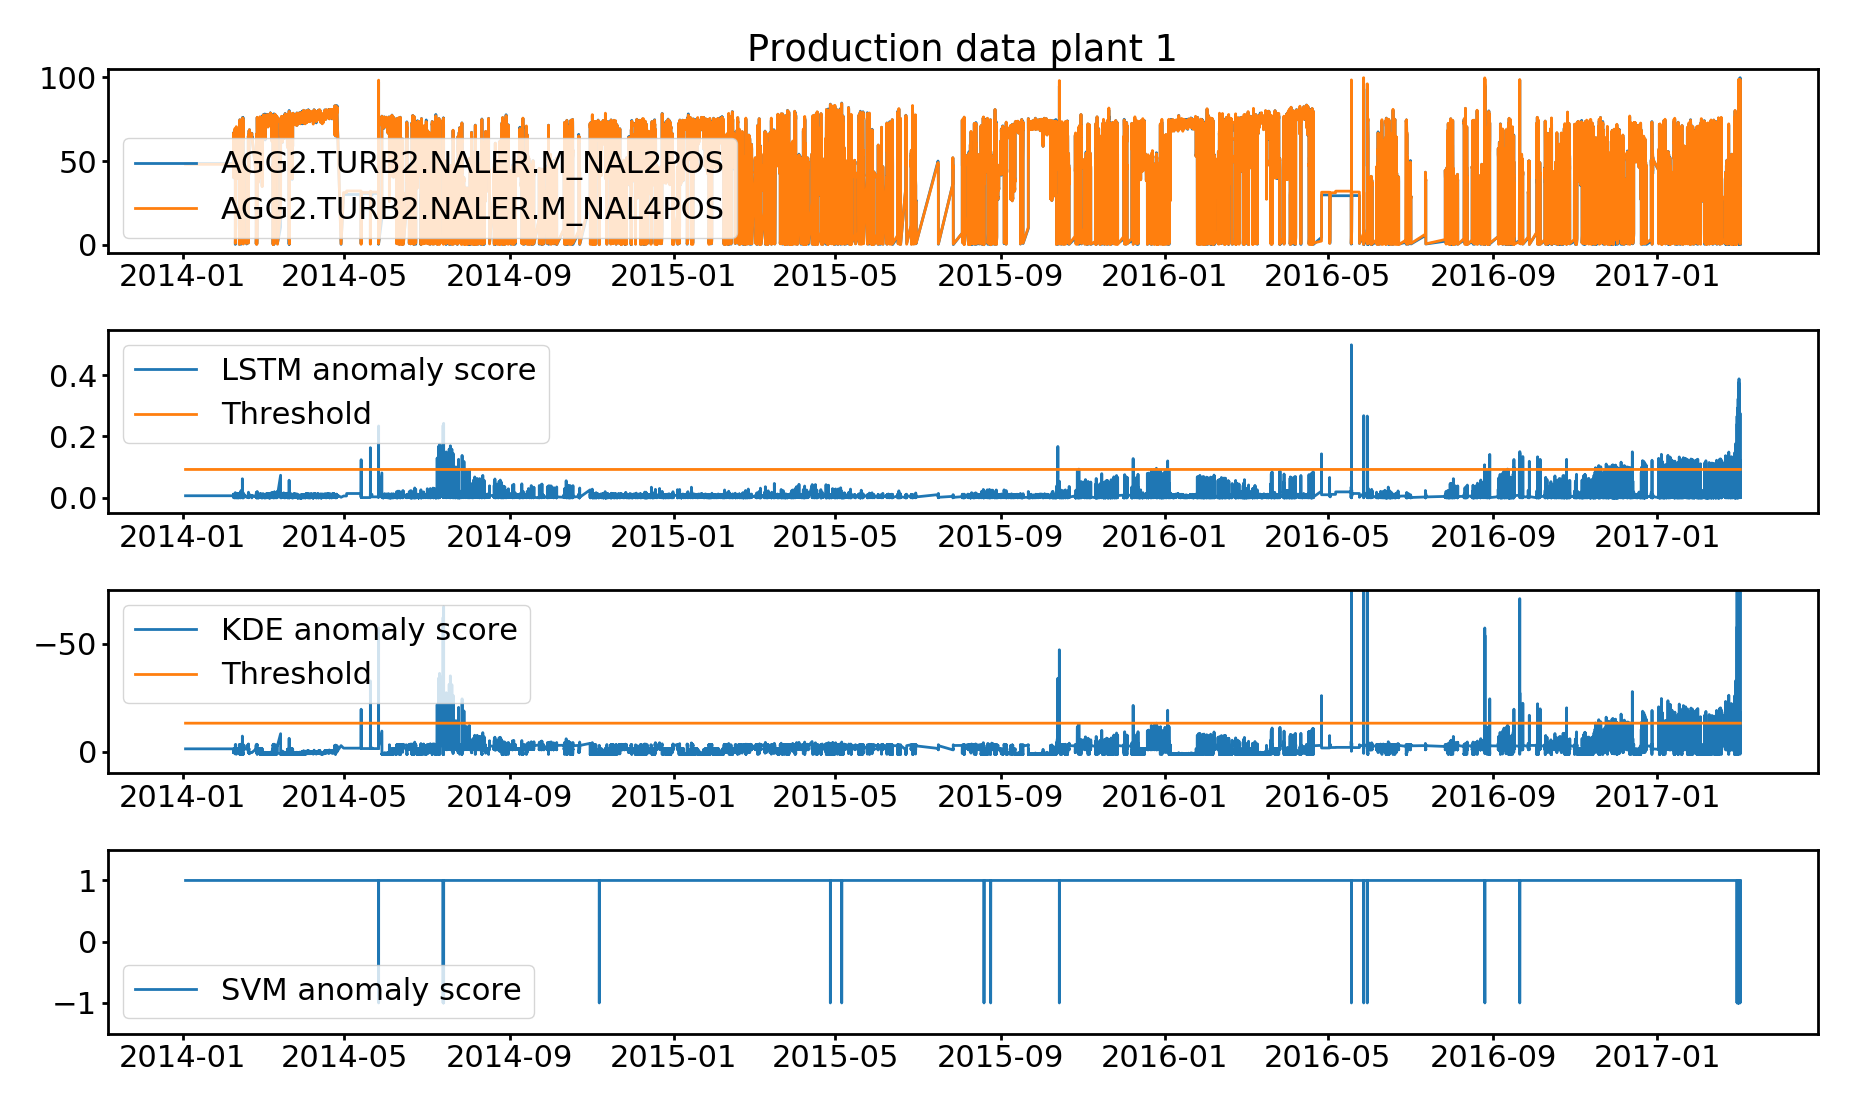
\includegraphics[width=\textwidth]{report/figures/analysis/plant2_train_short/production_data_anomaly.png}
            \caption{Anomaly results for the methods trained on training set 2 and evaluated on test case 1. For plot interpretation see Figure \ref{fig:anomaly_training_set1}.}
            \label{fig:plant2_short_prod_anomaly_score}
        \end{figure}
        Figure \ref{fig:plant2_short_prod_anomaly_score} shows the anomaly scores for test case 1, when training the methods on training set 2. Training set 1 and 2 are as mentioned approximately of the same size. The figure shows a very similar pattern for the two anomaly scorers to what was seen for training set 1. This could mean that both methods generalize well across plants, at least as long as the training sets are of similar size. 
        
        The biggest difference is seen in the OC SVM window, where some new samples are being classified as anomalies in 2015. This could show that OC SVM is more sensitive to the training data, as the data from 2015 seems to be the best data from this needle pair. However, looking at Figure \ref{fig:svm_2_outliers_stats_production} it becomes clear that the number of anomalies detected in 2015 is small, and that setting a threshold as mentioned in the previous section could classify them as false positives.  
        
        Table \ref{tab:trainining_plant2_short_stats} shows the anomaly statistics for the validation set and test case 1. It is clear that both scorers have a higher minimum and maximum values than what was seen when the methods were trained on training set 1. They are, however, very similar in magnitude. The mean values for both scorers are also changed, which could indicate that the score is simply biased. 
        \begin{table}[]
            \centering
            \begin{tabular}{ccccc}
                \toprule
                            & \textbf{KDE validation}  & \textbf{KDE case 1}     & \textbf{LSTM validation}     & \textbf{LSTM case 1}   \\ \midrule
                min         & -4.566        & -296.370           & 2.336e-05            & 2.336e-05         \\ 
                max         & 1.291         & 1.2905             & 4.047e-2             & 0.498             \\ 
                mean        & --0.518       & -1.493             & 4.976e-04            & 8.116e-3          \\ \bottomrule
            \end{tabular}
            \caption{Table comparing the statistics for the KDE and LSTM anomaly detectors on the validation and production data}
            \label{tab:trainining_plant2_short_stats}
        \end{table}
        \begin{figure}[h!]
            \begin{minipage}[b]{0.49\linewidth}
                \centering
                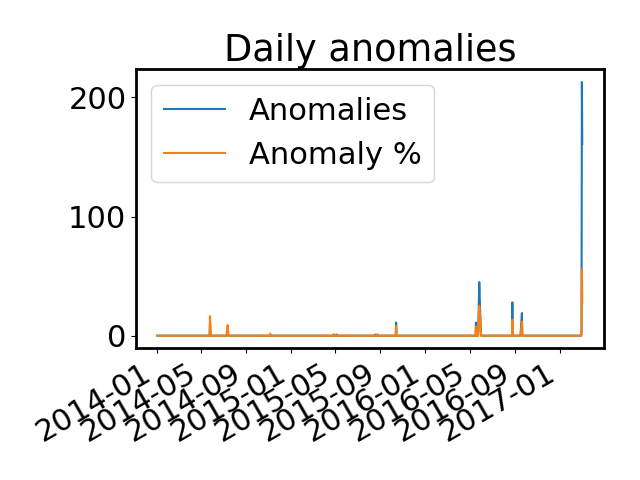
\includegraphics[width=\textwidth]{report/figures/analysis/plant2_train_short/daily_svm_outliers_production_small.png}
                \caption{Anomaly statistics for OC SVM on production data}
                \label{fig:svm_2_outliers_stats_production}
            \end{minipage}
            \hfill\vline\hfill
            \begin{minipage}[b]{0.49\linewidth}
                \centering
                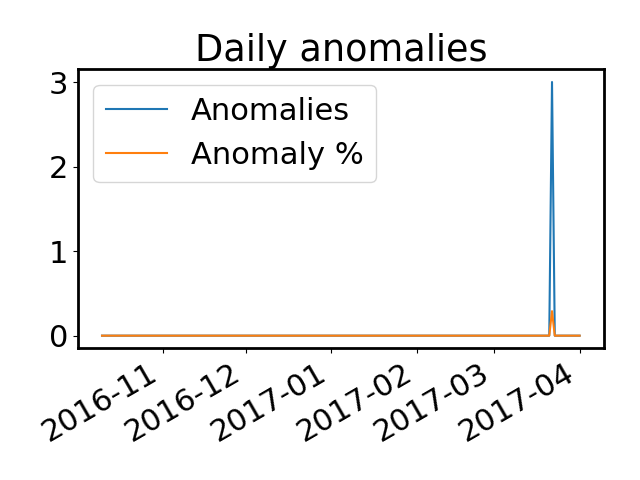
\includegraphics[width=\textwidth]{report/figures/analysis/plant2_train_short/daily_svm_outliers_artificial_small.png}
                \caption{Anomaly statistics for OC SVM on artificial data}
                \label{fig:svm_2_outliers_stats_artificial}
            \end{minipage}
        \end{figure}
        
        \begin{figure}[h!]
            \centering
            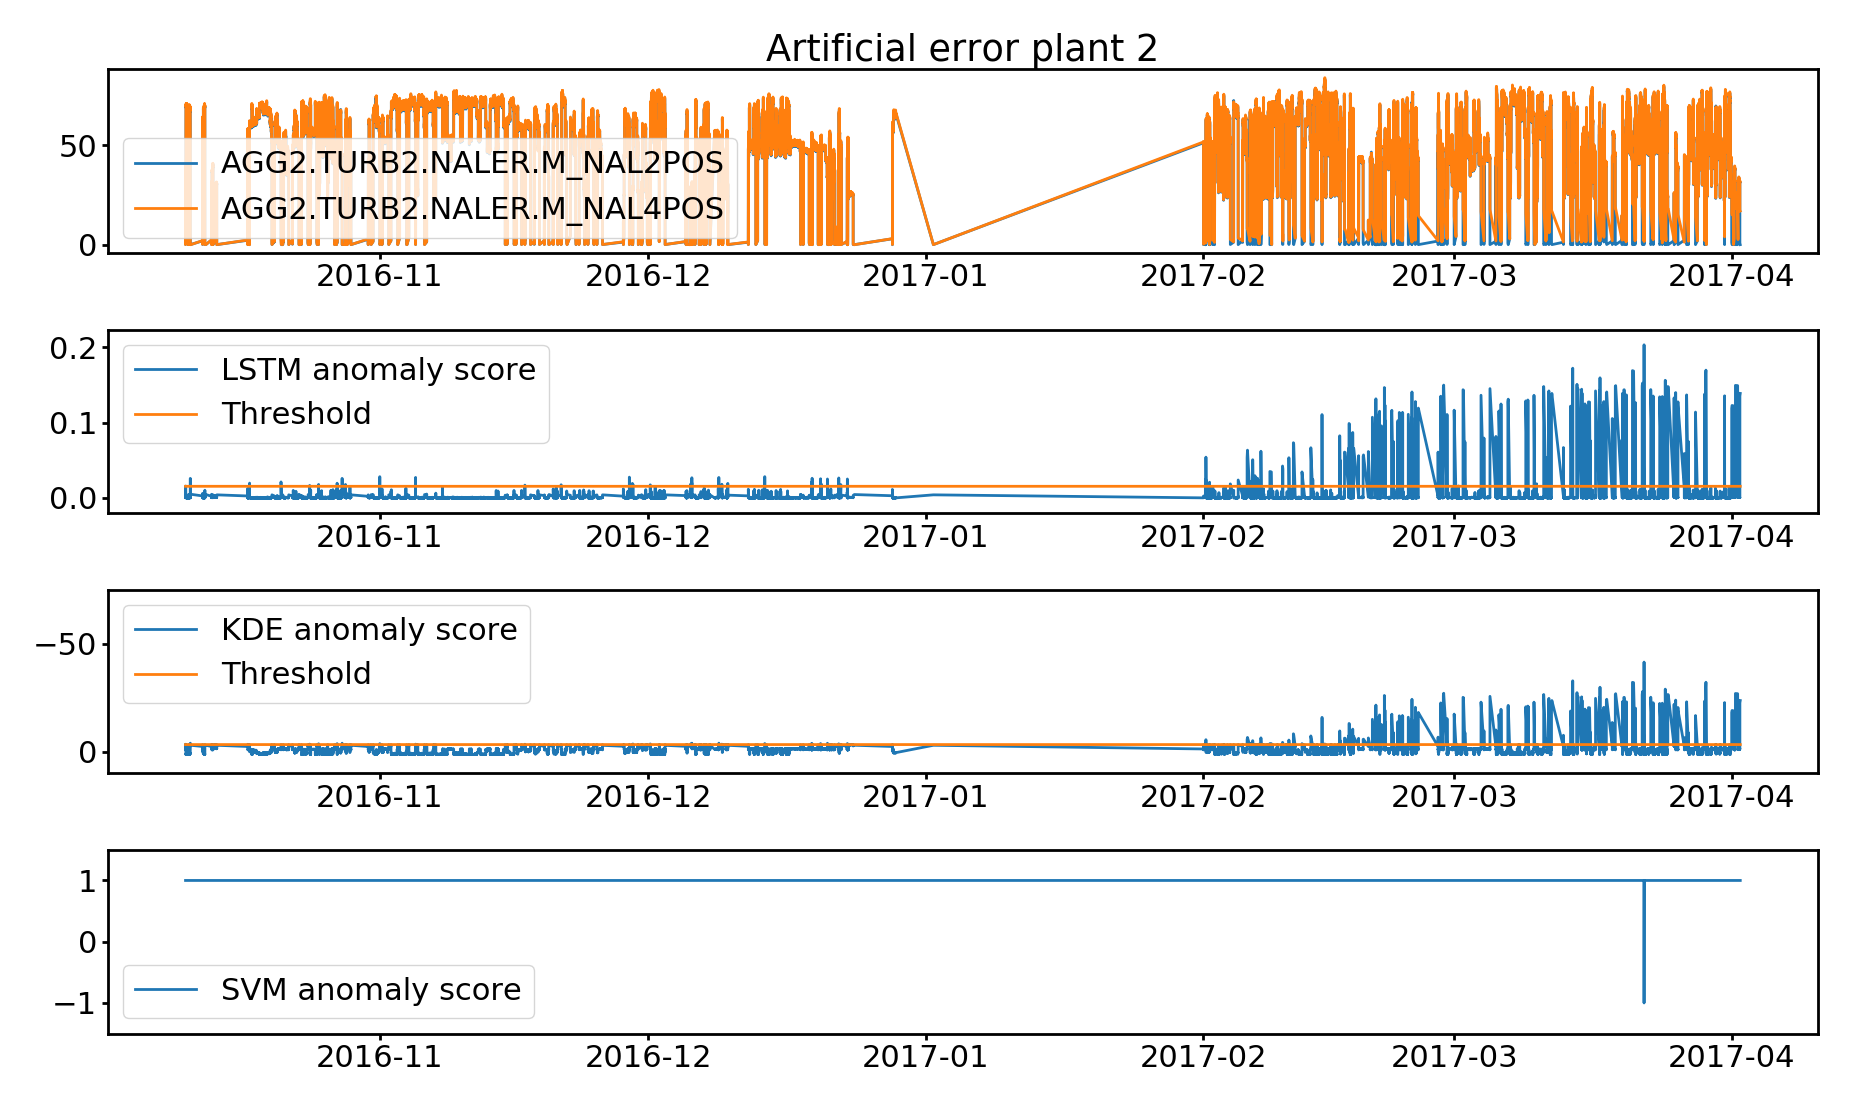
\includegraphics[width=\textwidth]{report/figures/analysis/plant2_train_short/artificial_data_anomaly.png}
            \caption{Anomaly results for the methods trained on training set 2 and evaluated on test case 2. For plot interpretation see Figure \ref{fig:anomaly_training_set1}.}
            \label{fig:plan2_short_arti_anomaly_score}
        \end{figure}
        Figure \ref{fig:plan2_short_arti_anomaly_score} shows the anomaly scores for the artificial data in test case 2. As with test case 1, both scorers behave very similar to what was seen for training set 1. Looking at the LSTM anomaly score in window two, one can verify that the anomaly score increases immediately after the error is applied. It can detect only small deviation from the normal operating pattern. The  KDE scorer also seems to pick up the artificial error faster than for training set 1. As the artificial error is added to process data from the same needle pair that is used for the data in training set 2, it is sensible that it is possible to detect the anomalies earlier than for training set 1. Looking at figure \ref{fig:plant2_short_prod_anomaly_score} one can see that the anomaly score for the artificial error is of the same magnitude as the score for test case 1 in the months before the incidents. 
        
        The OC SVM detector is, however, having problems detecting the anomalies, and only detects the sample that the two other detectors identify as the most anomalous. One possible explanation to this is that the parameters found in the hyperparameterization for the OC SVM do not generalize very well to new data, as the hyperparameterization was performed on data from plant 1. Figure \ref{fig:svm_2_outliers_stats_artificial} shows that the classifier is only classifying three samples as anomalous. The plot for the anomaly scores of the validation set can be found in appendix \ref{appendix:training_case2}, in addition, boundary plots for the OC SVM classifier, KDE scorer and learning history plots for the LSTM scorer can be found there.
        
        
    
    \subsection{Training set 3, test case 1 and 2}
        \begin{figure}
            \centering
            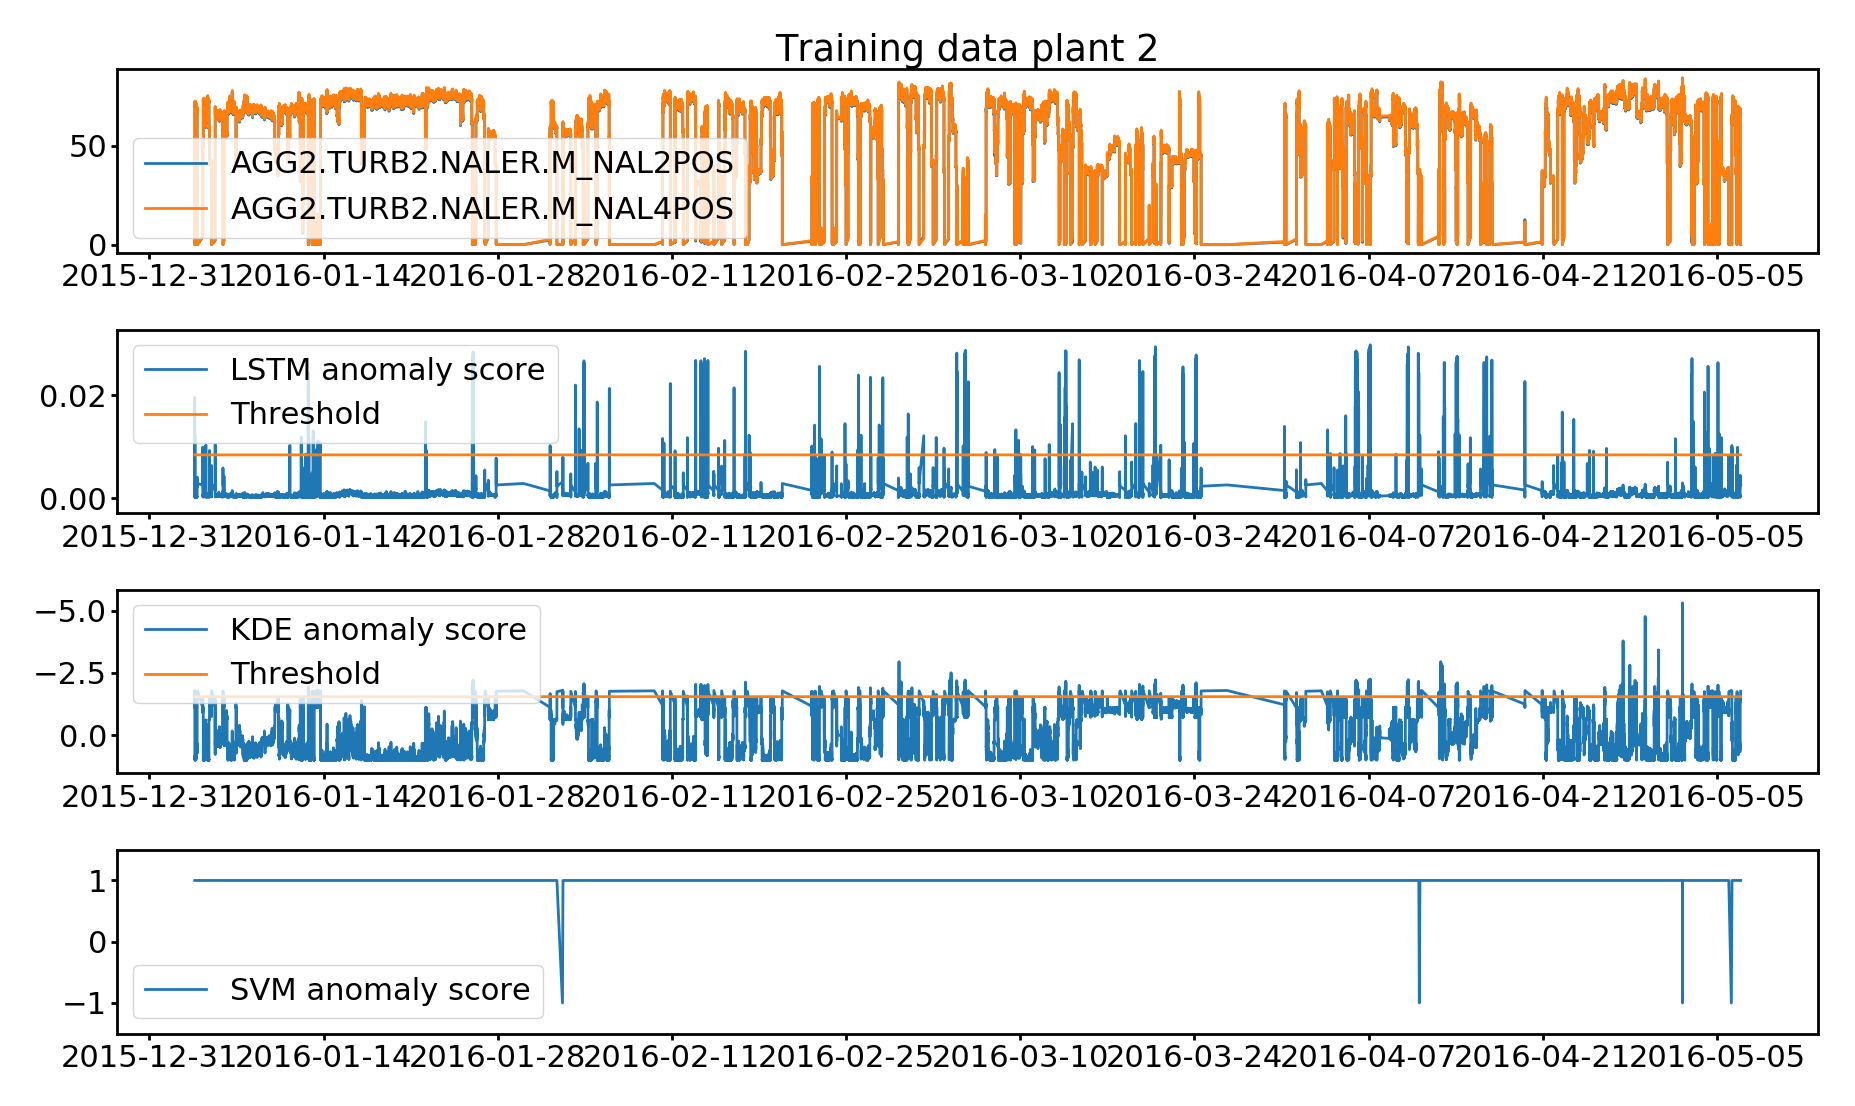
\includegraphics[width=\textwidth]{report/figures/analysis/plant2_train_long/training_data_anomaly.png}
            \caption{Anomaly results for the methods trained on training set 3 evaluated on training set 3. For plot interpretation see Figure \ref{fig:anomaly_training_set1}.}
            \label{fig:anomaly_training_set3}
        \end{figure}
        Figure \ref{fig:anomaly_training_set3} shows training set 3, and how the different methods evaluate the training data. The magnitude of the anomaly scores for the two scorers is between the scores for training set 1 and 2.  The OC SVM evaluates the most anomalies of all the training sets. As this training set is 10 times larger than the two other, this further strengthens the claim that the OC SVM hyperparameters are sensitive to the training data. 
    
        \begin{figure}[h!]
            \centering
            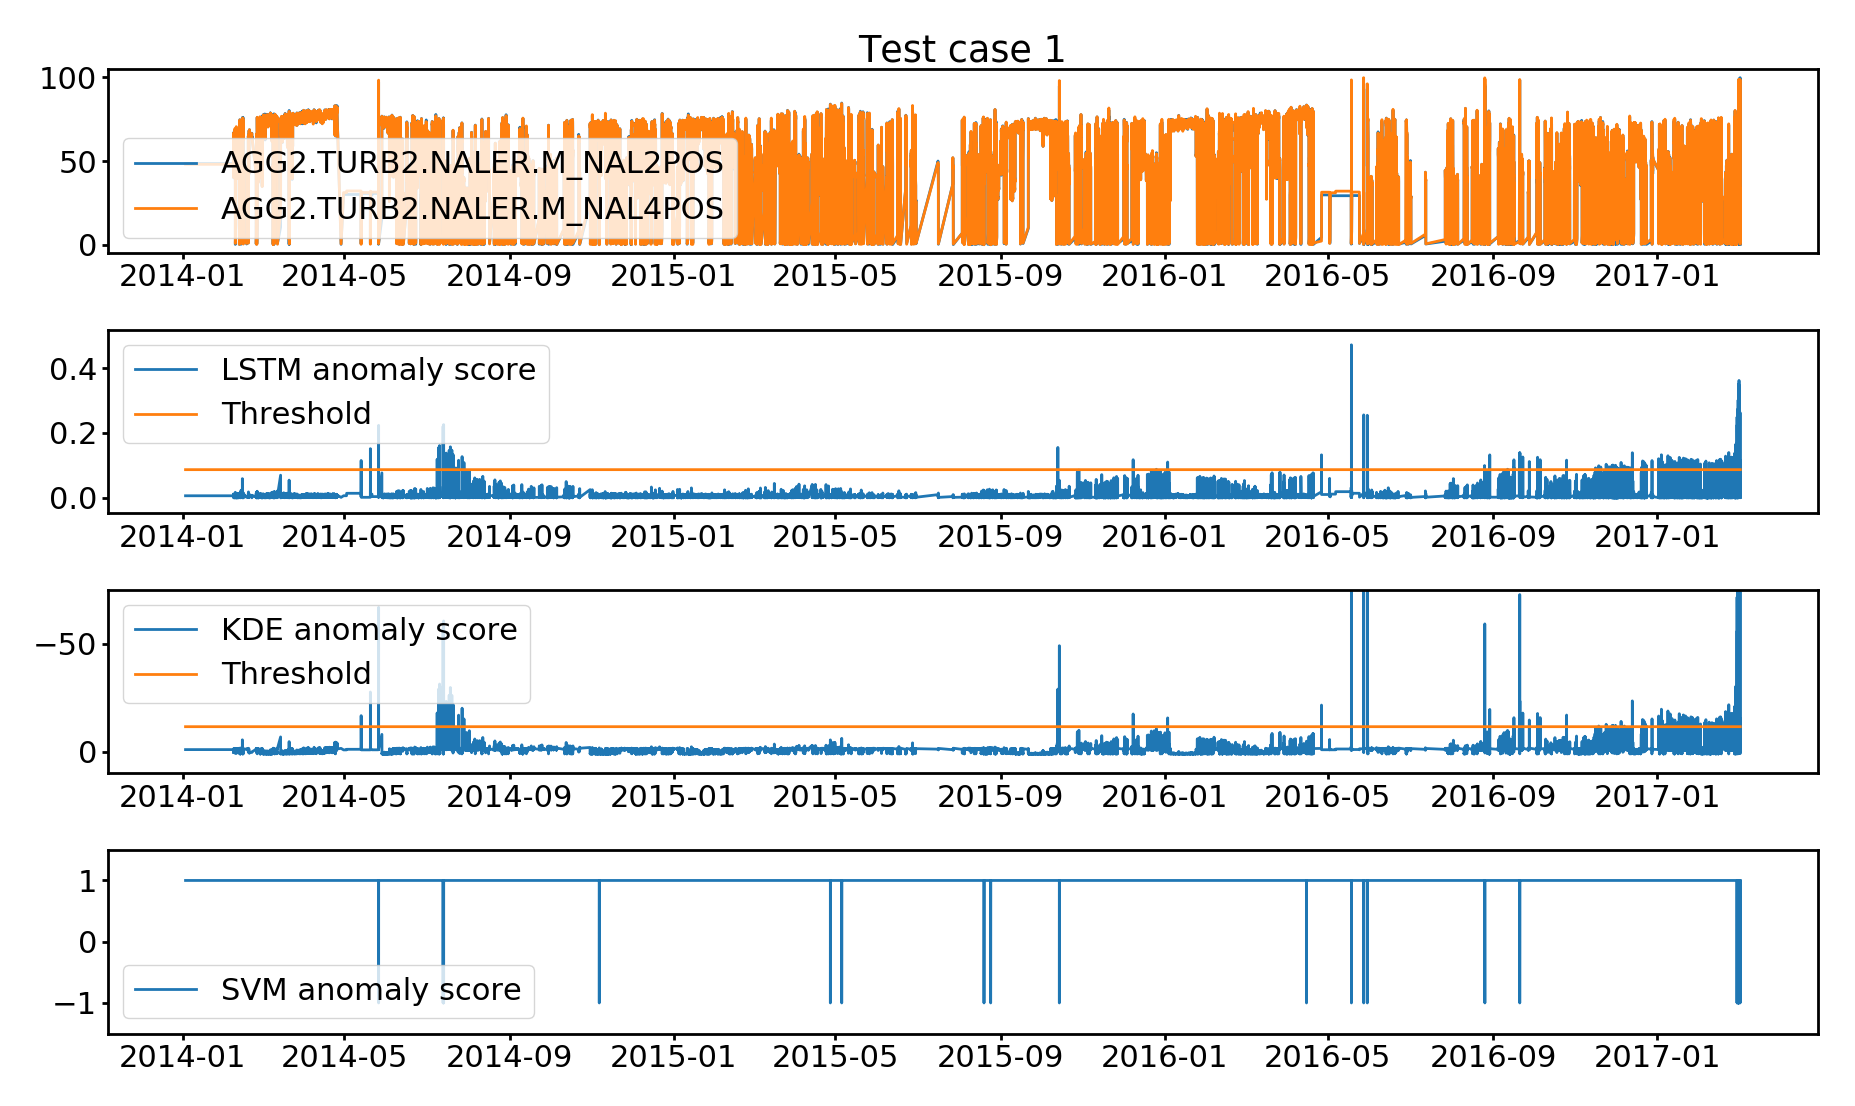
\includegraphics[width=\textwidth]{report/figures/analysis/plant2_train_long/production_data_anomaly.png}
            \caption{Anomaly results for the methods trained on training set 3 and evaluated on test case 1. For plot interpretation see Figure \ref{fig:anomaly_training_set1}.}
            \label{fig:plant2_lomg_prod_anomaly_score}
        \end{figure}
        Figure \ref{fig:plant2_lomg_prod_anomaly_score} shows the anomaly scores and classifications for test case 1 when trained on training set 3. The scorers evaluate anomalies very similar to what was seen for training set 1 and 2. Both scorers detect a rising trend of abnormal data towards the reported incident in March 2017. The anomaly scores for the data from the day of the incident is very high for both scorers, as was seen in the two previous cases as well. The OC SVM classifier is classifying test case 1 very similar to what was seen for training set 2, as is verified by Figure \ref{fig:svm_3_outliers_stats_production}. Adding more data from plant 2 did not fix the issue with what appears to be false positives in the data sampled in 2015. 
        
        \begin{figure}[h!]
            \begin{minipage}[b]{0.49\linewidth}
                \centering
                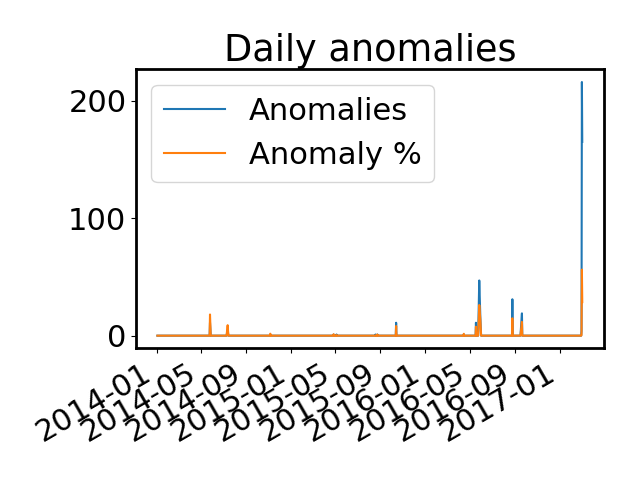
\includegraphics[width=\textwidth]{report/figures/analysis/plant2_train_long/daily_svm_outliers_production_small.png}
                \caption{Anomaly statistics for one class SVM on production data}
                \label{fig:svm_3_outliers_stats_production}
            \end{minipage}
            \hfill\vline\hfill
            \begin{minipage}[b]{0.49\linewidth}
                \centering
                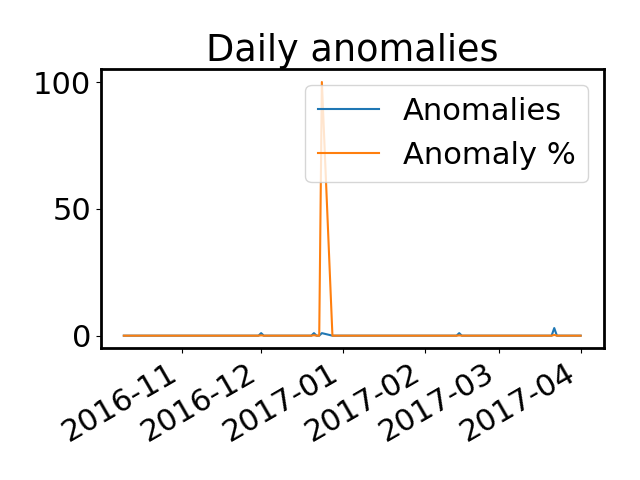
\includegraphics[width=\textwidth]{report/figures/analysis/plant2_train_long/daily_svm_outliers_artificial_small.png}
                \caption{Anomaly statistics for one class SVM on artificial data}
                \label{fig:svm_3_outliers_stats_artificial}
            \end{minipage}
        \end{figure}
        
        Table \ref{tab:trainining_plant2_long_stats} show the statistics for the LSTM and KDE detectors, the statistics are similar to what was seen in the previous training sets. Early stopping stopped the LSTM scorer after only 20 epochs, where the two previous sets ran for 134. When running the LSTM for 134 epochs, the performance of the LSTM scorer was much worse than for the previous training sets. This could indicate that training set 2 holds the same information as training set 3, but as training set 3 has more samples, the algorithm does not need to iterate over the entire set as many times. Early stopping is used to avoid overfitting on the training data, and the poor performance when running for 134 epochs on set 3, is most likely due to overfitting. The fact that the two other methods appear to evaluate test case 1 similar for both training set 2 and 3, further strengthens this claim. If the added data in set 3 has a different distribution than the one in training set 2, this would have been caught by KDE and one class SVM.     
        \begin{table}[]
            \centering
            \begin{tabular}{ccccc}
                \hline
                            & \textbf{KDE validation}  & \textbf{KDE case 1}     & \textbf{LSTM validation} & \textbf{LSTM case 1}   \\ \midrule
                min         & -2.755    & -277.804              & 2.559e-05         & 2.796e-05         \\ 
                max         & 0.999     & 0.9995                & 3.597e-2          & 0.471             \\ 
                mean        & -0.366   & -1.167                 & 6.709e-04         & 7.651e-03          \\ \bottomrule
            \end{tabular}
            \caption{Table comparing the statistics for the KDE and LSTM anomaly detectors on the validation and production data}
            \label{tab:trainining_plant2_long_stats}
        \end{table}




        % Figure \ref{fig:plan2_short_arti_anomaly_score} shows the anomaly scores for the artificial data. As with the production data from plant 1 both the KDE and LSTM detectors behave very similar to what was seen for training case 1. Looking at the LSTM anomaly score in window two, one can verify that the detector can track the artificial error from the date it is applied whereas for training case 1 it took a long time before the anomaly score indicated something abnormal. The one class SVM detector is, however, having problems detecting the anomalies, and only detects the sample that the two other detectors identify as the most abnormal. Note that the training case here is based on normal data from plant 2. It seems like the parameters found in the hyperparameterization of the one class SVM does not generalize very well to new data.
        \begin{figure}[h!]
            \centering
            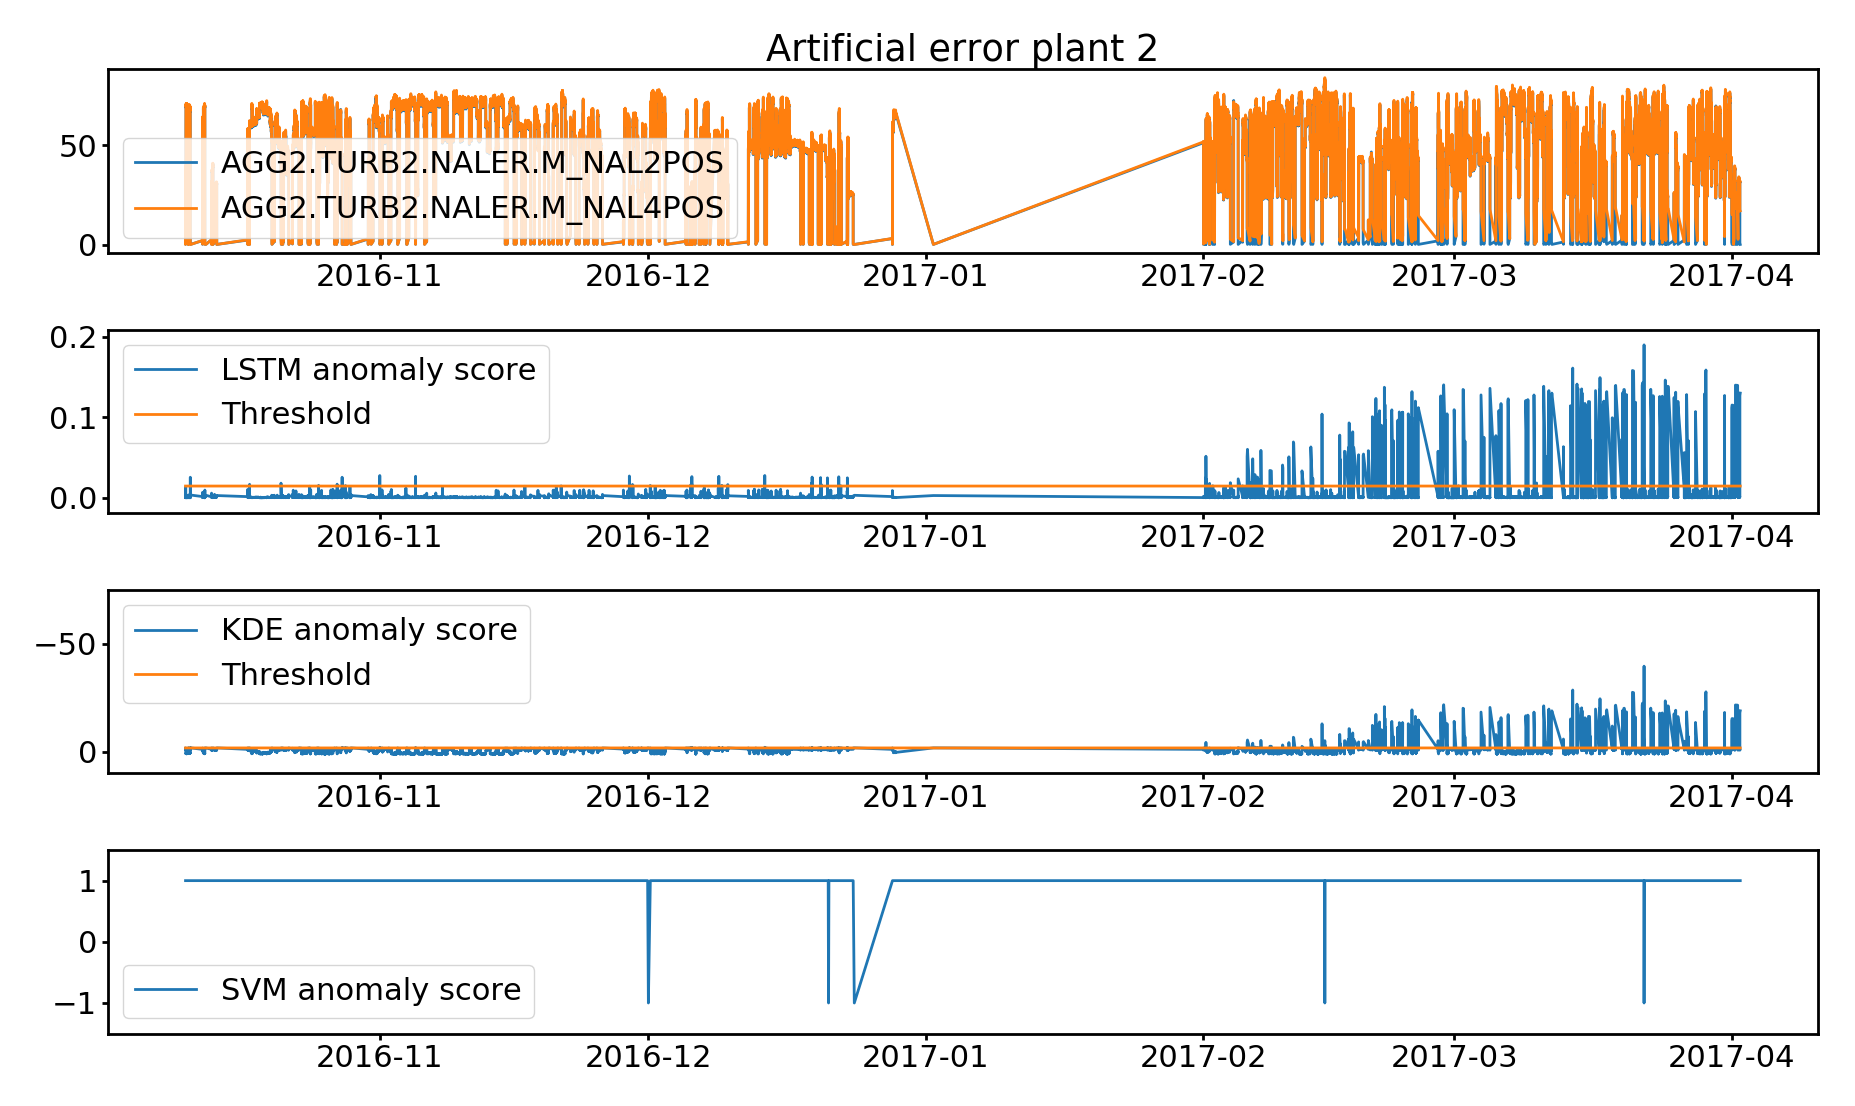
\includegraphics[width=\textwidth]{report/figures/analysis/plant2_train_long/artificial_data_anomaly.png}
            \caption{Anomaly results for the methods trained on training set 3 and evaluated on test case 2. For plot interpretation see Figure \ref{fig:anomaly_training_set1}.}
            \label{fig:plan3_long_arti_anomaly_score}
        \end{figure}
        Figure \ref{fig:plan3_long_arti_anomaly_score} shows the anomaly scores for test case 2. As for test case 1, one can verify that the scorers behave more or less equal to what was seen for training set $2$. The OC SVM classifier is detecting anomalies in the normal test data, and it is only able to classify data from one day during the artificial error as anomalous. Figure \ref{fig:svm_3_outliers_stats_artificial} shows that for a day in the end of December, all samples are evaluated as anomalies. This is most likely due to only one sample being stored right after midnight. The fact that training set 3 yields the poorest performance for the OC SVM, further strengthens the assumption that the algorithm is sensitive to the combination of hyperparameters and training data. The plot for the anomaly scores on the validation set can be found in appendix \ref{appendix:training_case3}, in addition, boundary plots for the SVM classifier, KDE scorer and learning history plots for the LSTM scorer can be found there.
        
    
    
    \subsection{Comparing the methods for all training sets, on test case 1}
        \begin{figure}[h!]
            \centering
            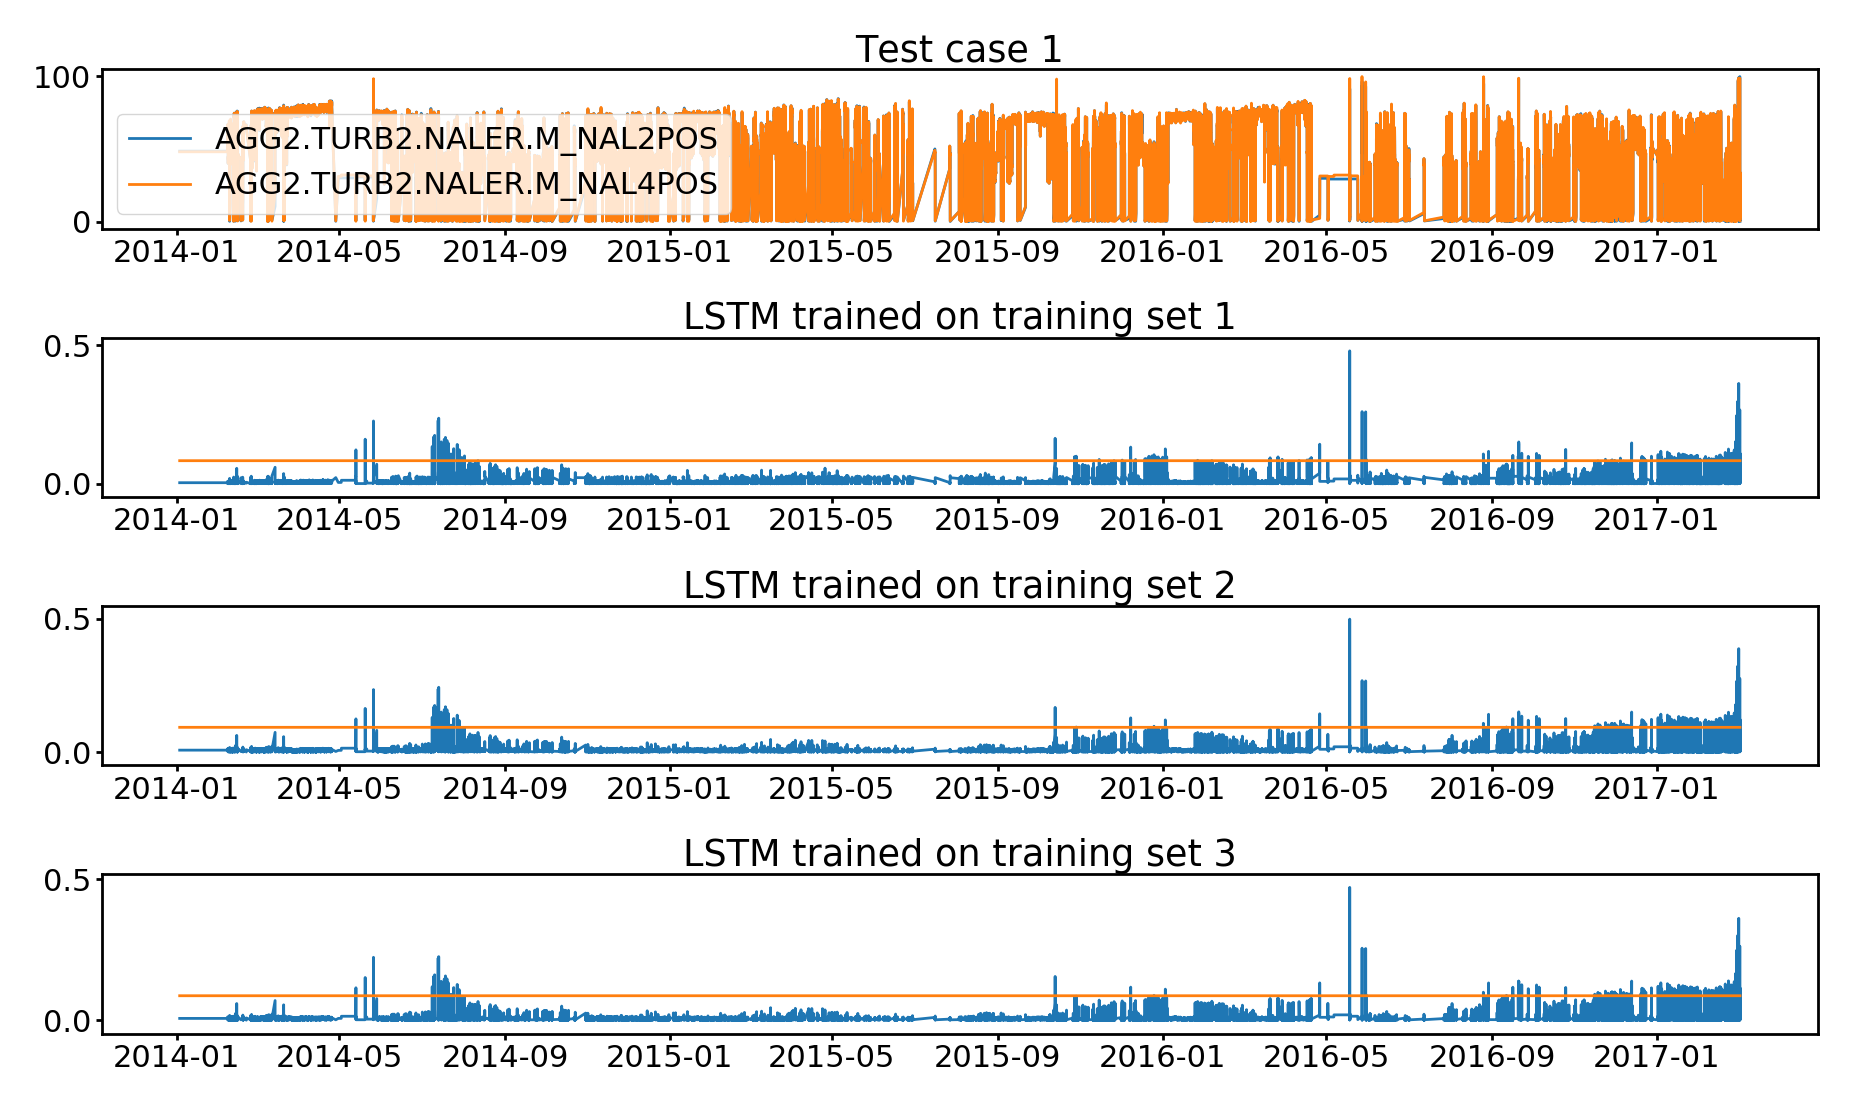
\includegraphics[width=\textwidth]{report/figures/analysis/training_cases/lstm_training_cases.png}
            \caption{The anomaly score for the three LSTM scorers tested on test case 1, is seen in the three lower subplots. The upper subplot shows the needle positions on top of each other. The orange line indicates the 0.1\% most extreme scores.}
            \label{fig:lstm_training_cases}
        \end{figure}
        To simplify comparing the performance of the different methods new plots are created that shows how the different methods evaluate the production data in test case 1, for all three training sets. Figure \ref{fig:lstm_training_cases} show how test case 1 is evaluated by the three LSTM scorers. It is clear that all the scorers perform very similar. This shows that the method works well for both large and smaller training sets. All scores indicate a growing anomaly trend towards the incident in 2017, but the scorers for training set 2 and 3 show an increasing anomaly trend earlier than the scorer for set 1. A theory for why this is happening is that the training data used in set 1 is sampled right after maintenance, while the training sets from plant 2 are sampled after years of operation. This means that minor deviations between the needles that could be normal after some time of use is seen as anomalous for the scorer trained on set 1 while this is seen as normal when set 2 and 3 are used for training. However, deploying any of the three scorers at the plant could have warned about an increase in anomalous observations, that could have identified the anomalous trend before it is becoming too extreme. 
        
        \begin{figure}[h!]
            \centering
            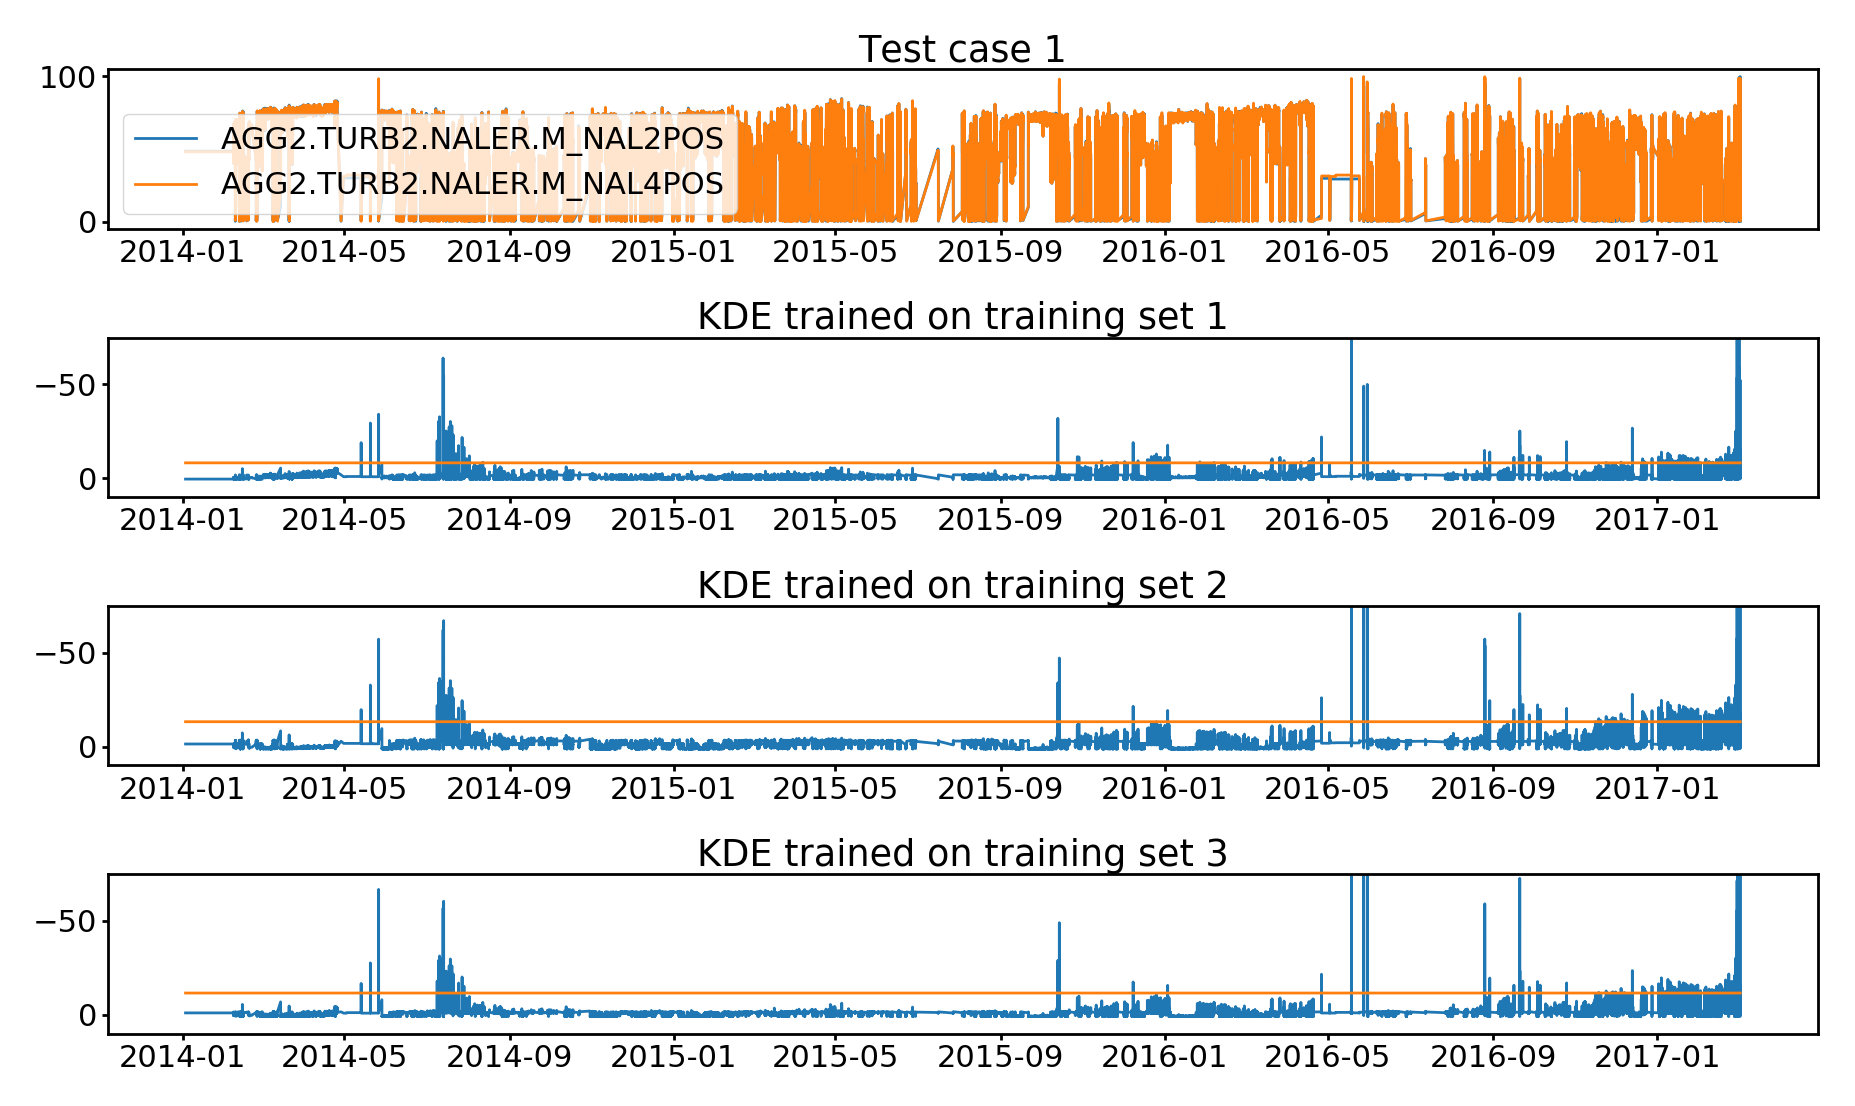
\includegraphics[width=\textwidth]{report/figures/analysis/training_cases/kde_training_cases.png}
            \caption{The anomaly score for the three KDE scorers tested on test case 1, is seen in the three lower subplots. The upper subplot shows the needle positions on top of each other. The orange line indicates the 0.1\% most extreme scores.}
            \label{fig:kde_training_cases}
        \end{figure}
        Figure \ref{fig:kde_training_cases} shows how the different KDE scorers compare. All three scorers evaluate test case 1 very similar. The scorer from training set 2 gives the highest anomaly scores for the data leading up to the incident. As with the LSTM scorers, set 2 and set 3 appears to perform slightly better than set 1. All three scorers are able to detect the growing number of abnormal data seen towards March 2017. Notice that the score is limited to -75 to enable the reader to see the smaller trends, as the extreme values go below -250, making interpreting the plot very hard.
        
        \begin{figure}[h!]
            \centering
            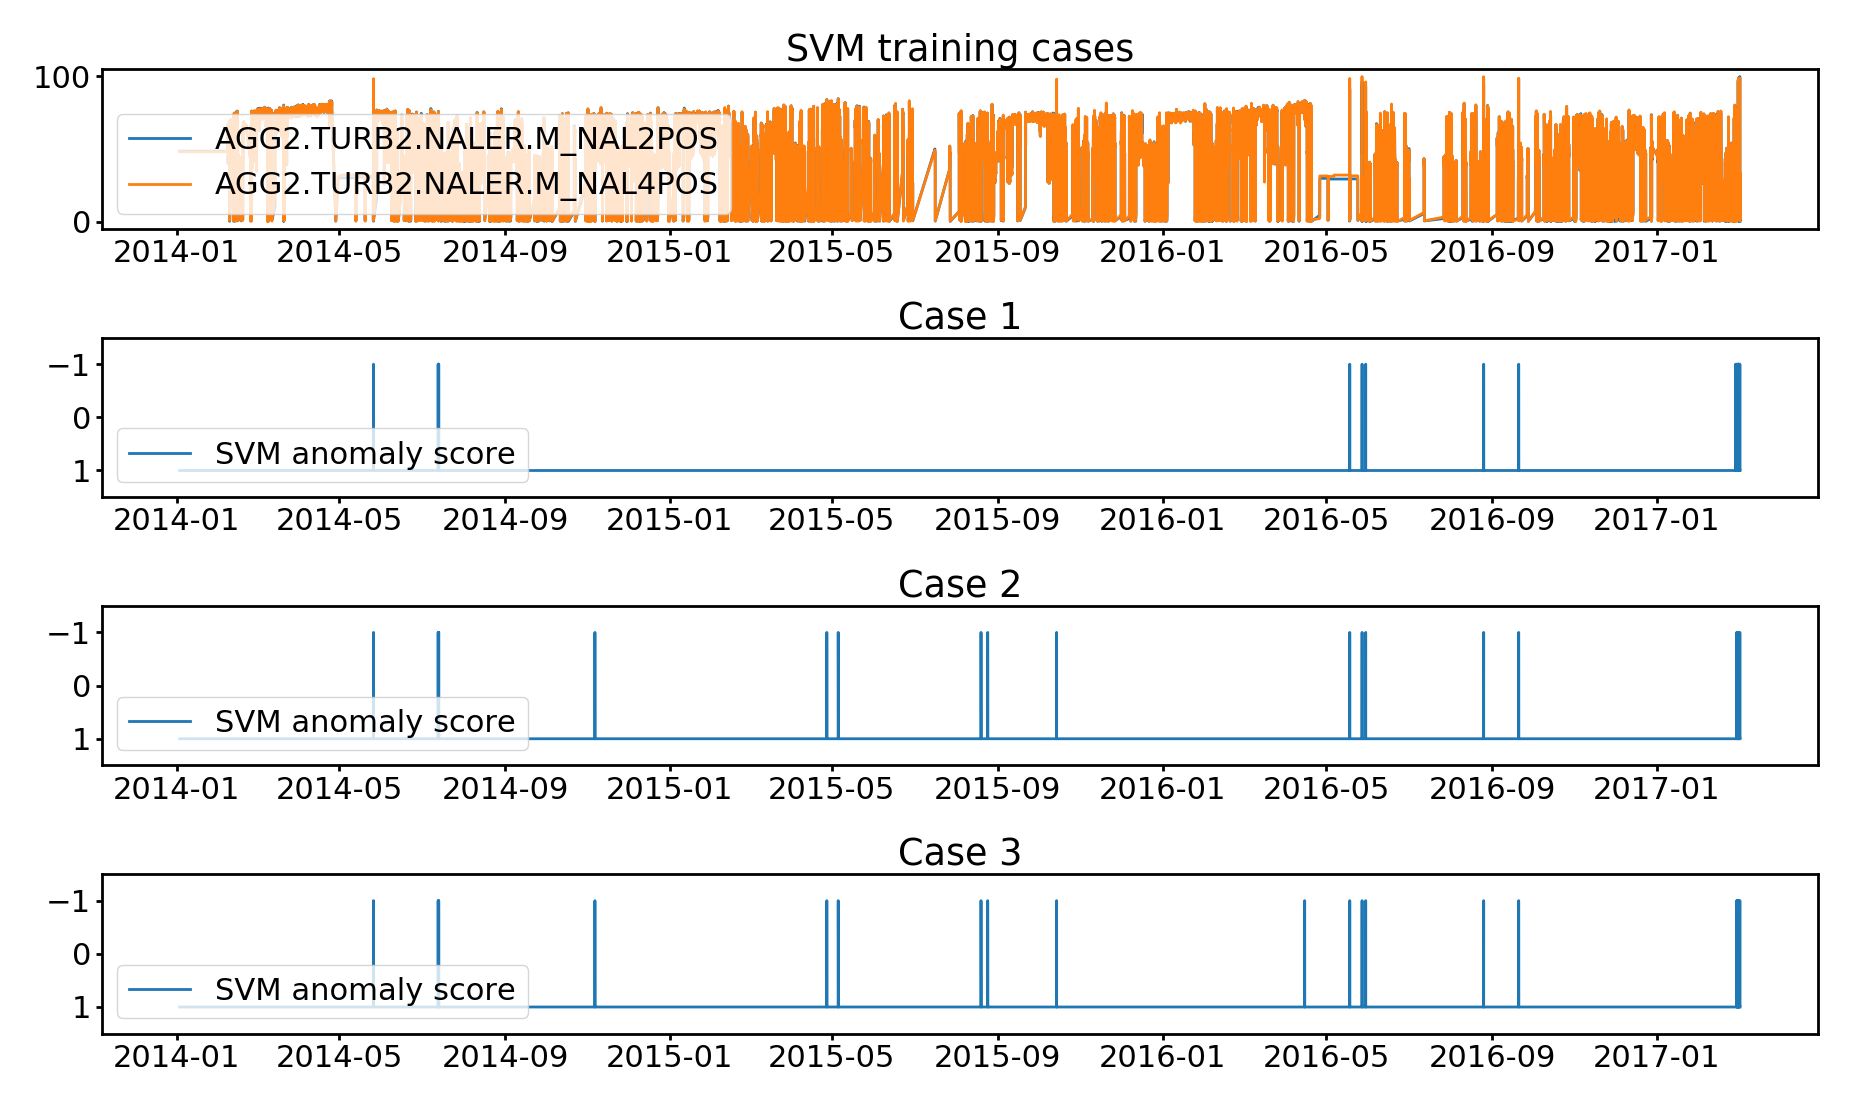
\includegraphics[width=\textwidth]{report/figures/analysis/training_cases/svm_training_cases.png}
            \caption{The anomaly classification for the three OC SVM classifiers tested on test case 1, are seen in the three lower subplots. The upper subplot shows the needle positions on top of each other. Normal data = 1, anomalous data = -1}
            \label{fig:svm_training_cases}
        \end{figure}
        Finally, Figure \ref{fig:svm_training_cases} show the three different one class SVM classifiers. As with the two previous methods, there is little difference between set 2 and 3. This is the only method that appears to perform best when trained on data from plant 1. However, there is very little difference in the classifications, and when using the percentage of daily anomalies, one can easily separate the data from the incident with the other. This method is harder to spot trends with, and with the current parameterization, it is hard to find a way this method can be used as an early warning system for the incident seen in March 2017. This makes sense, as this method predicts all data as either normal or anomalous, and hence include an extra step compared to KDE and LSTM, which gives a score that the user need to interpret. Hence using this method would require less of the user, but more tuning and testing to ensure correct behavior. 
        
    
    \subsection{Test case 3 and 4}
        As the production data from test case 1 only contained one reported anomaly, the methods are tested on two start failures in test case 3 and 4. The results for the methods trained on training set 2 is seen in Figure \ref{fig:start_up_t1} and \ref{fig:start_up_t2}. In Figure \ref{fig:start_up_t1} one can see that the reported start failure from 10.12.2014 is given a high anomaly score for both scorers. The OC SVM classifier is not able to detect the start failure, and also appears to classify data from November as an anomaly wrongly. Notice that the magnitude of the scores is lower than what was seen for the most extreme samples from test case 1, it is, however, very similar to the magnitude seen for the artificial error.
        \begin{figure}
            \centering
            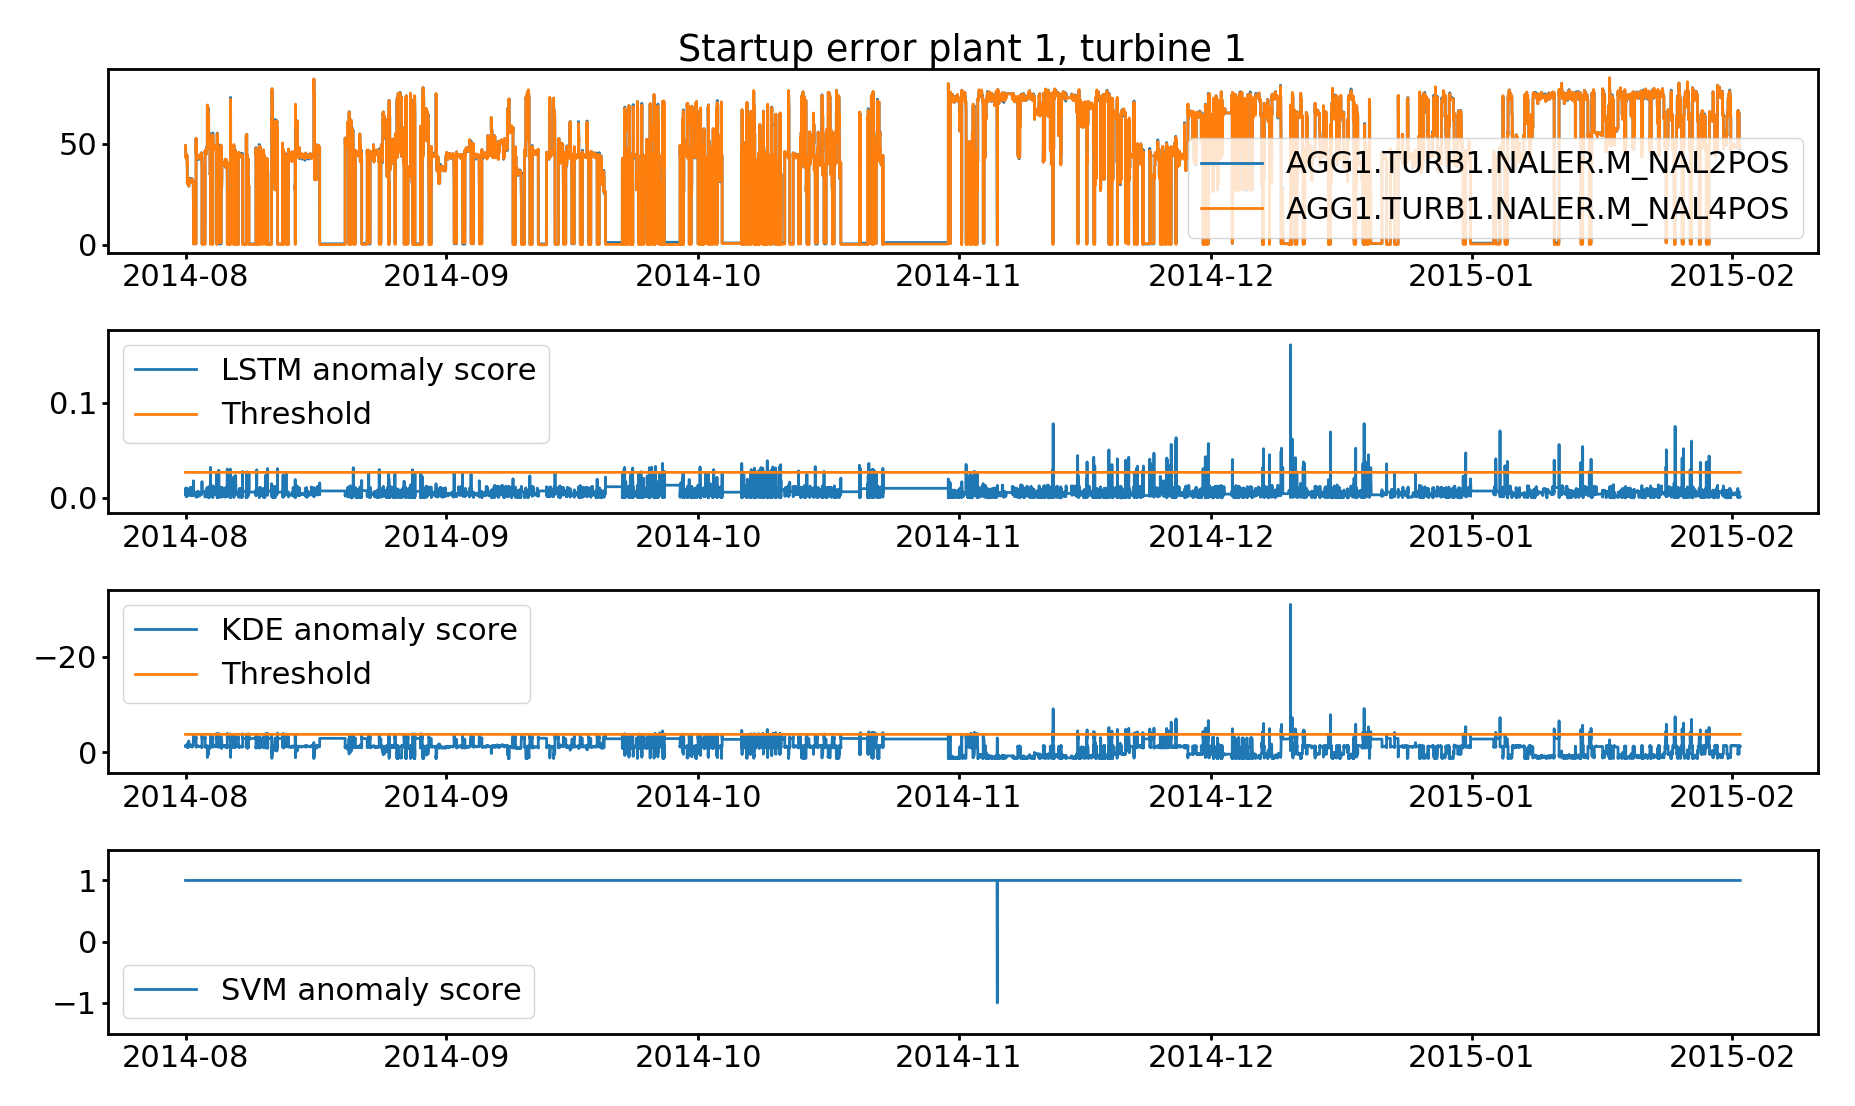
\includegraphics[width=\textwidth]{report/figures/analysis/startup_errors/t1_n2_n4_startup_error_anomaly_score_2_long.png}
            \caption{Anomaly results for the methods trained on training set 2 and evaluated on test case 3. How to interpret the figure can be seen in Figure \ref{fig:anomaly_training_set1}.}
            \label{fig:start_up_t1}
        \end{figure}
        In Figure \ref{fig:start_up_t2}, the start failure from case 4 is analyzed. The scoreres evaluate the start failure to be more anomalous than the start failure in case 3, as the magnitude of the scores are doubled. This is reasonable when looking at Figure \ref{fig:start_failure_turb1} and \ref{fig:start_failure_turb2}, where the scatterplot for turbine 1 clearly deviates more than the scatterplot for turbine 2. The OC SVM classifer is also able to detect the start failure.
        \begin{figure}
            \centering
            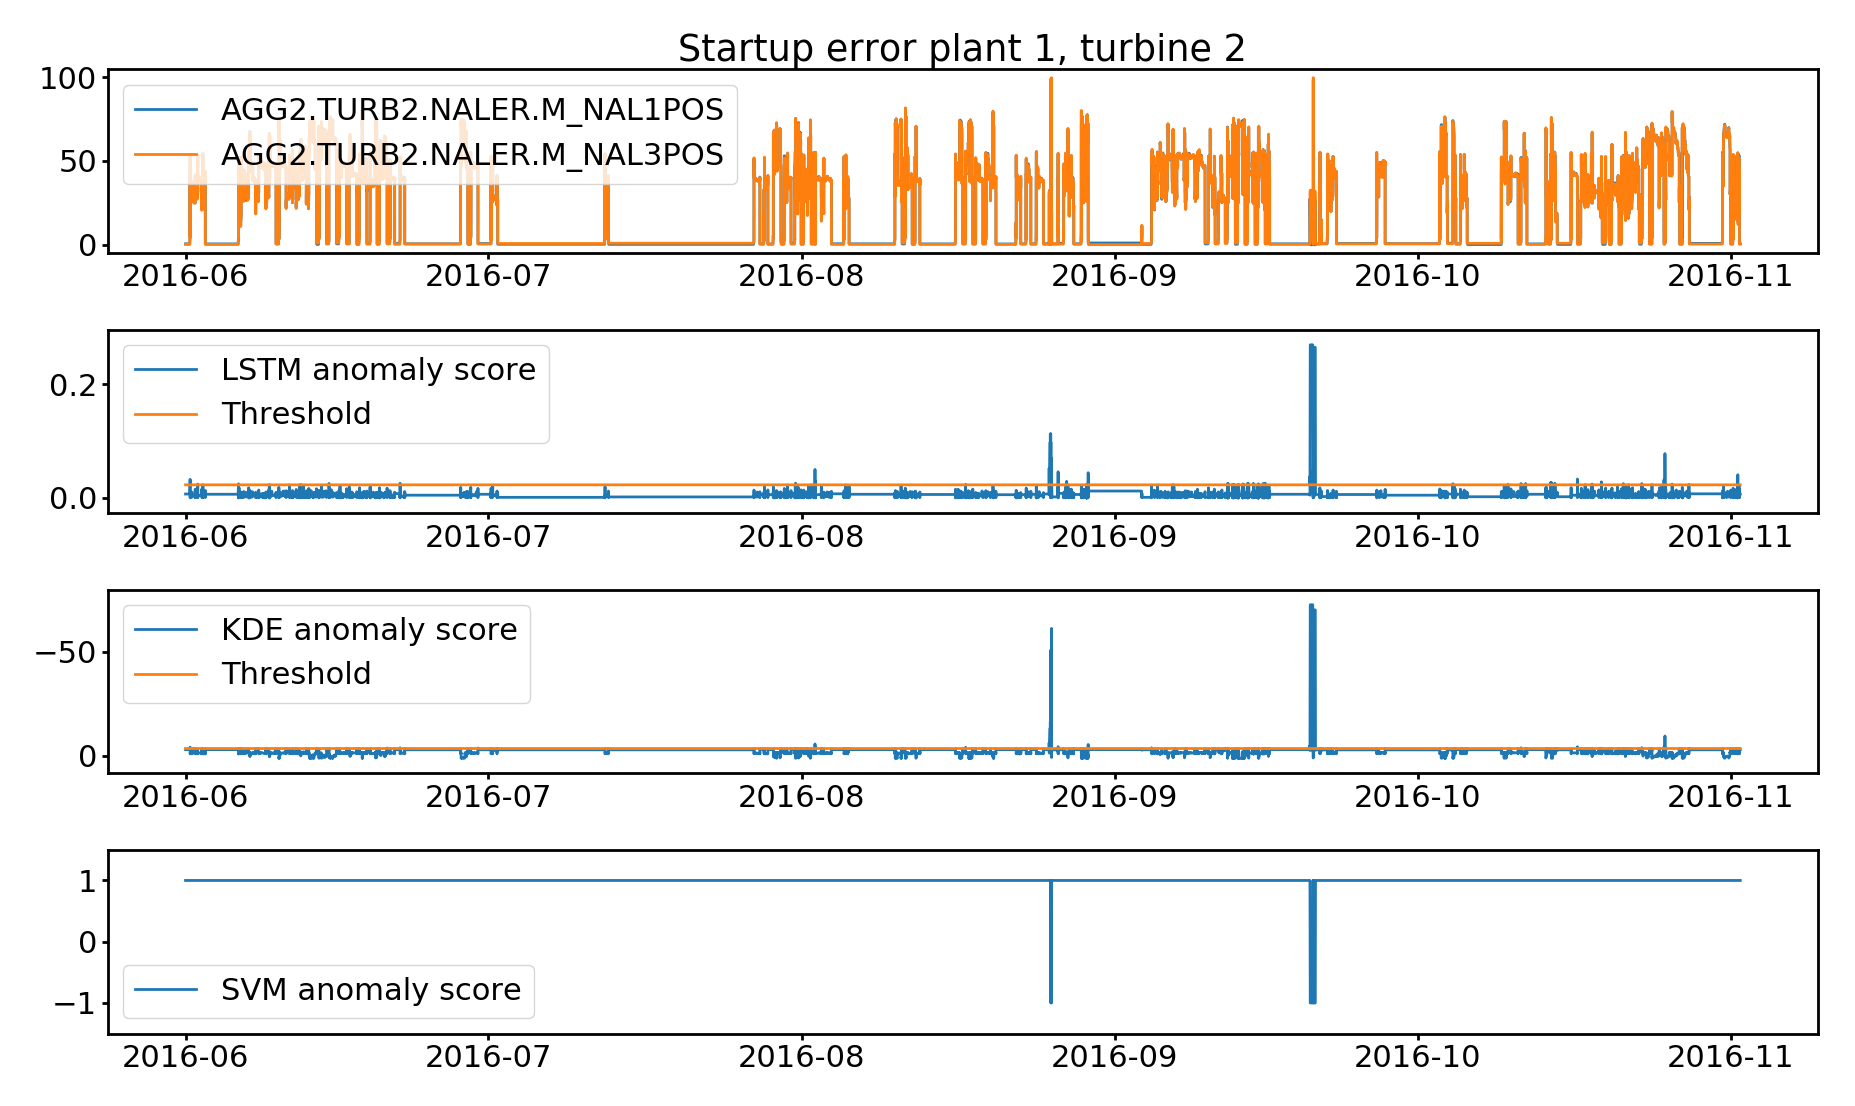
\includegraphics[width=\textwidth]{report/figures/analysis/startup_errors/t2_n1_n3_startup_error_anomaly_score_2_long.png}
            \caption{Anomaly results for the methods trained on training set 2 and evaluated on test case 4. How to interpret the figure can be seen in Figure \ref{fig:anomaly_training_set1}.}
            \label{fig:start_up_t2}
        \end{figure}
        The figures for the two other training sets can be found in appendix \ref{appendix:startup_failure}. They are not included in this section, due to very similar performance as the one seen for training set 2. 
    
    
    
    
    
    
    
    
    
    
    
    
    
    
    
    
    
    
    
    
    %     \begin{figure}
    %         \centering
    %         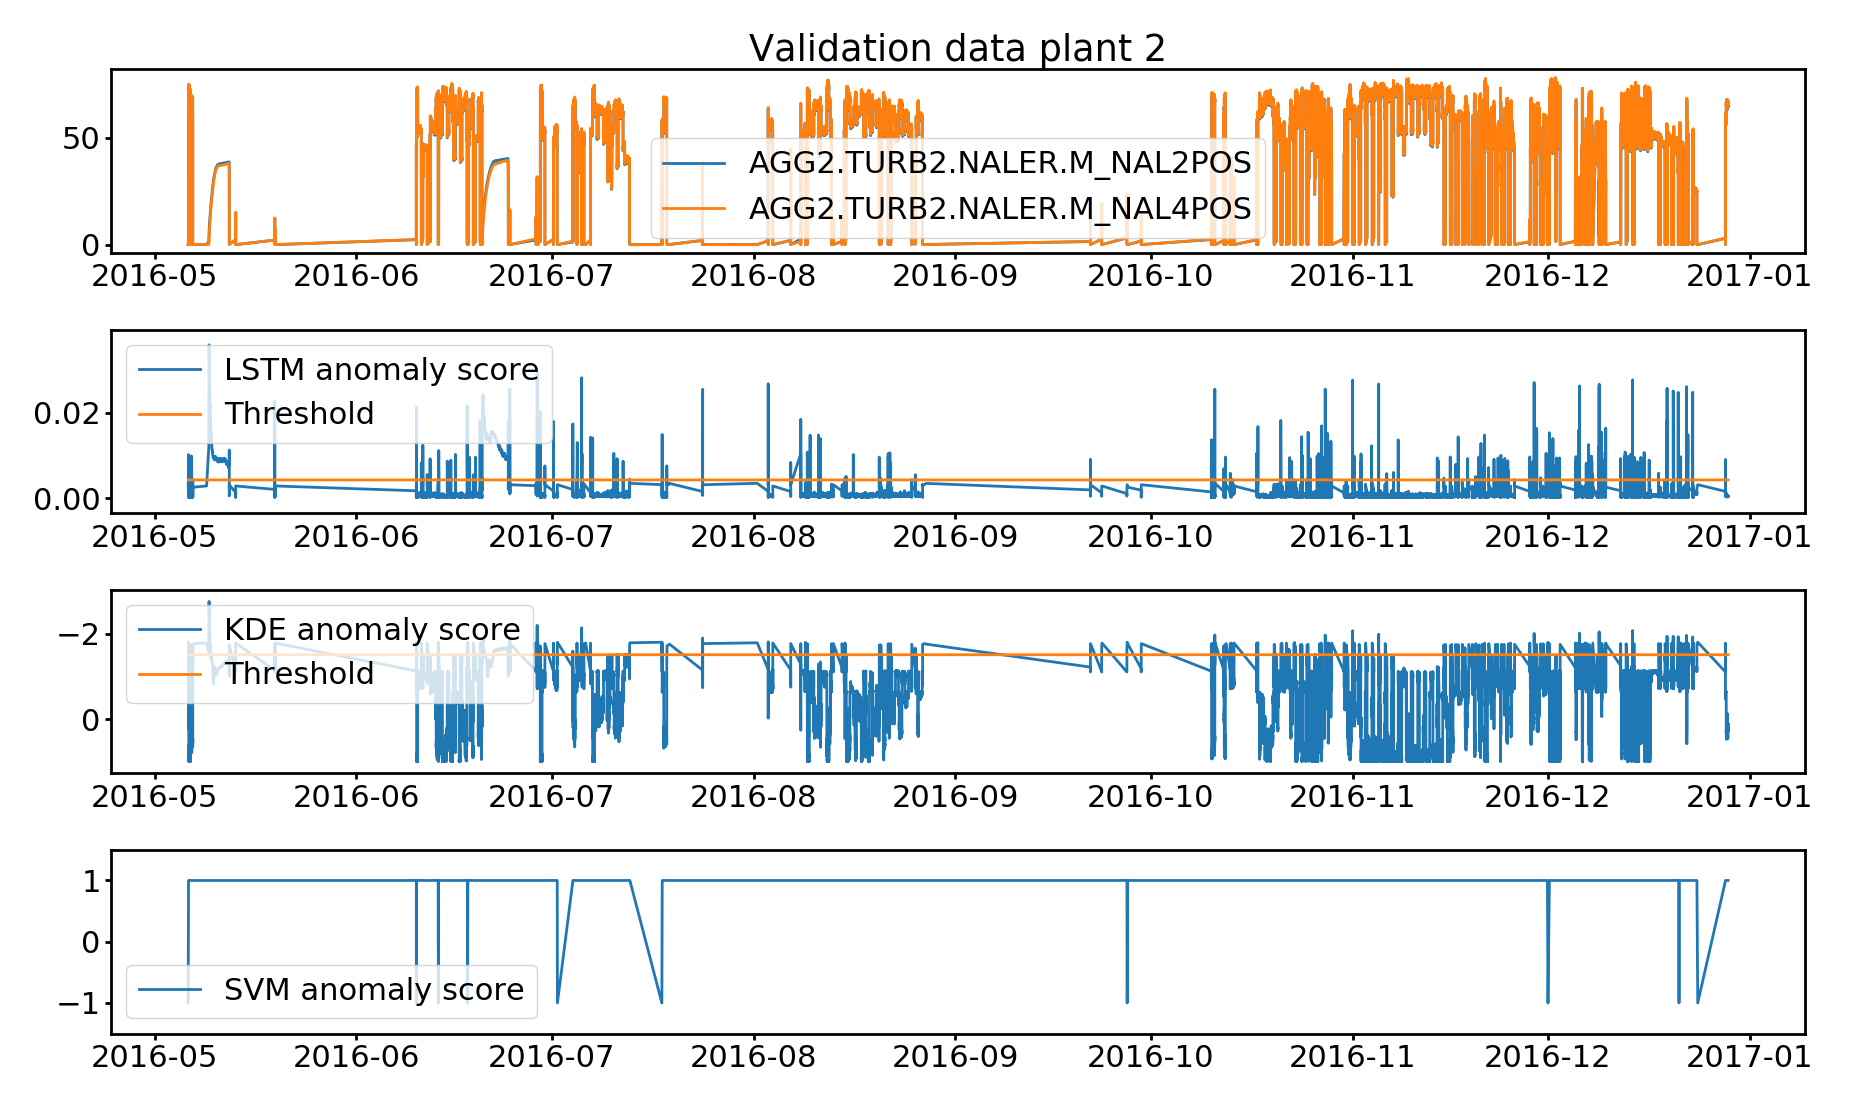
\includegraphics[width=\textwidth]{report/figures/analysis/plant2_train_long/test_data_anomaly.png}
    %         \caption{Anomaly score for the plant 2 test set, detectors trained on plant 2 long training set}
    %         \label{fig:plant2_long_test_anomaly_score}
    %     \end{figure}
        
    %     \begin{figure}
    %         \centering
    %         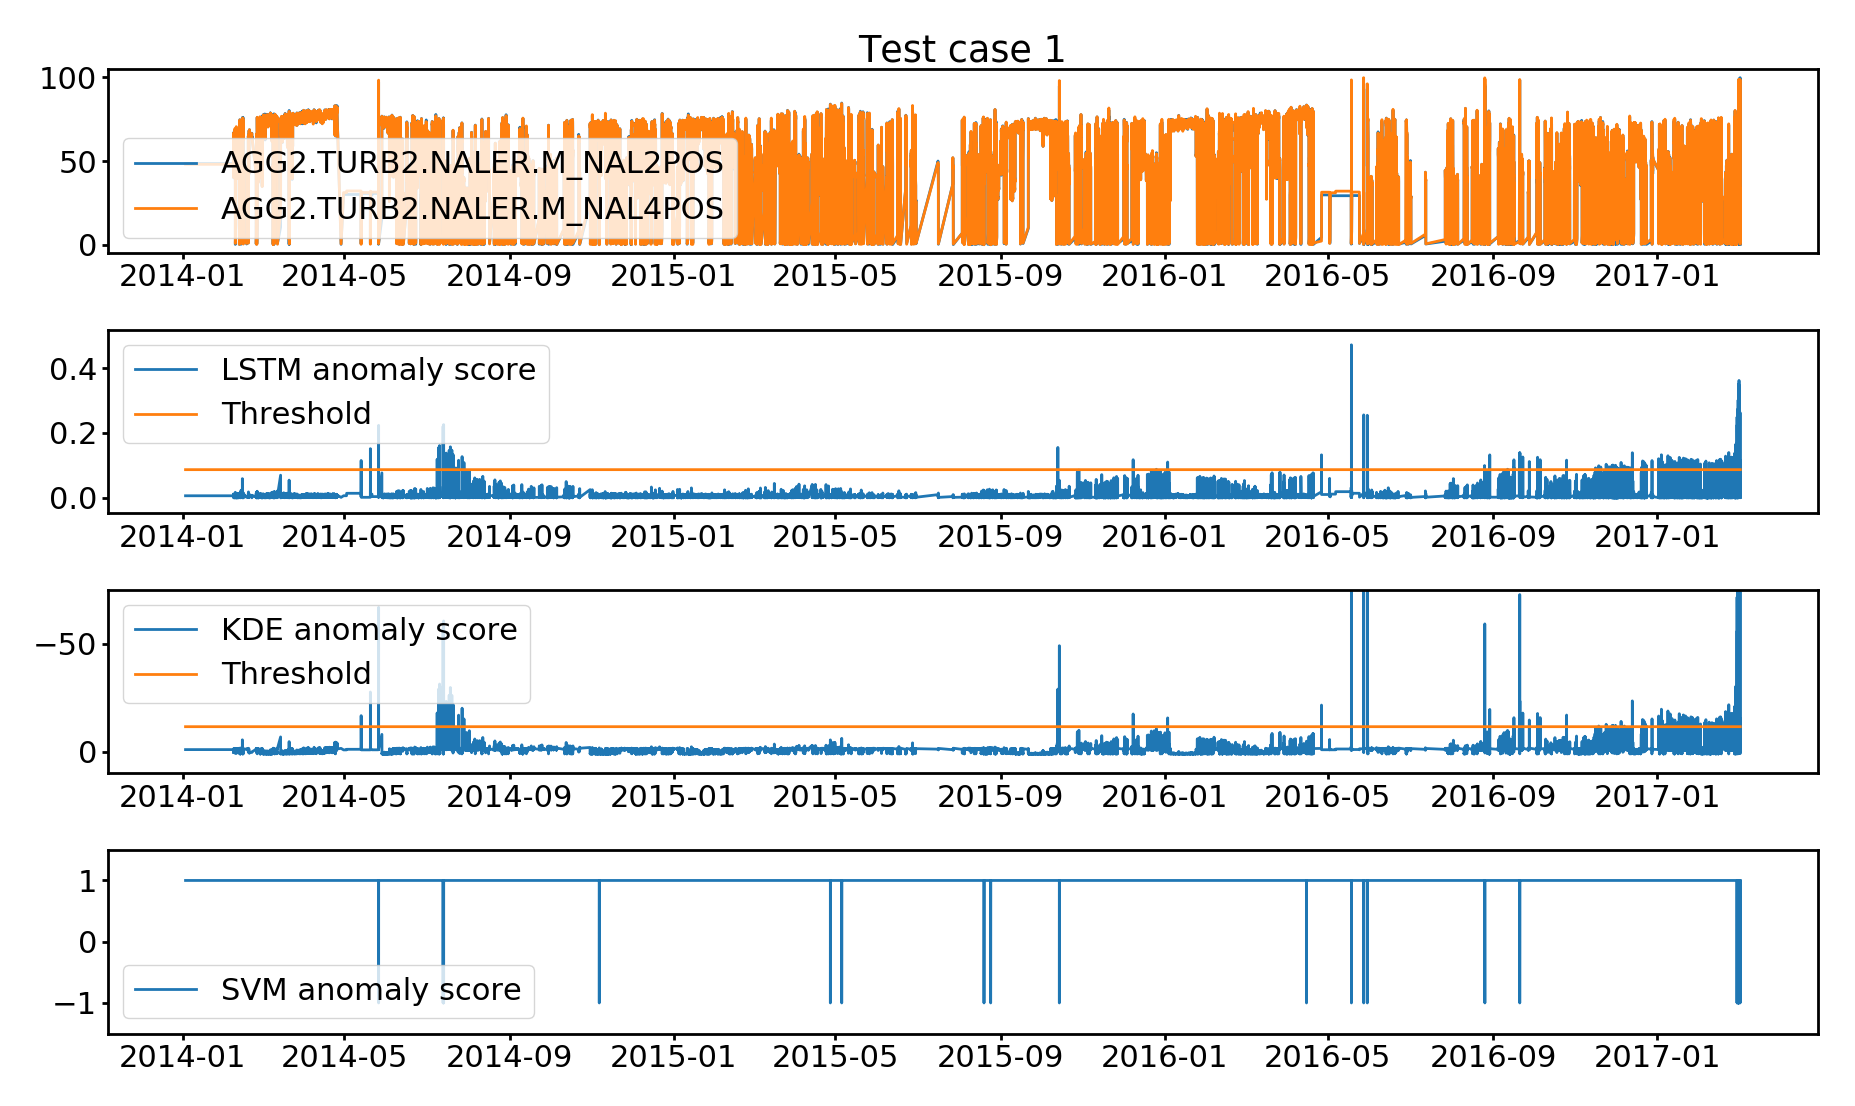
\includegraphics[width=\textwidth]{report/figures/analysis/plant2_train_long/production_data_anomaly.png}
    %         \caption{Anomaly score for the plant 1 production set, detectors trained on plant 2 long training set}
    %         \label{fig:plant2_long_production_anomaly_score}
    %     \end{figure}
    
    
    
    %     % \begin{table}[]
    %     %     \centering
    %     %     \begin{tabular}{|c|c|c|}
    %     %         \hline
    %     %         Test        & KDE       & LSTM  \\ \hline
    %     %         min         & -2.755    & 4.024e-05 \\ \hline
    %     %         max         & 0.999    & 0.0024   \\ \hline
    %     %         mean        & -0.366   & 0.000223  \\ \hline
    %     %     \end{tabular}
    %     %     \caption{Table of statistics for the test data for plant 2 long detector}
    %     %     \label{tab:production_stats_plant1train}
    %     % \end{table}
        
    %     % \begin{table}[]
    %     %     \centering
    %     %     \begin{tabular}{|c|c|c|}
    %     %         \hline
    %     %         Production          & KDE       & LSTM  \\ \hline
    %     %         min                 & -277.804   & 2.013e-05 \\ \hline
    %     %         max                 & 0.9987    & 0.0.0457   \\ \hline
    %     %         mean                & -1.1697    & 0.0.000807  \\ \hline
    %     %     \end{tabular}
    %     %     \caption{Table of statistics for the production data for plant 2 long detector}
    %     %     \label{tab:production_stats_plant1train}
    %     % \end{table}

    %     \begin{figure}
    %         \centering
    %         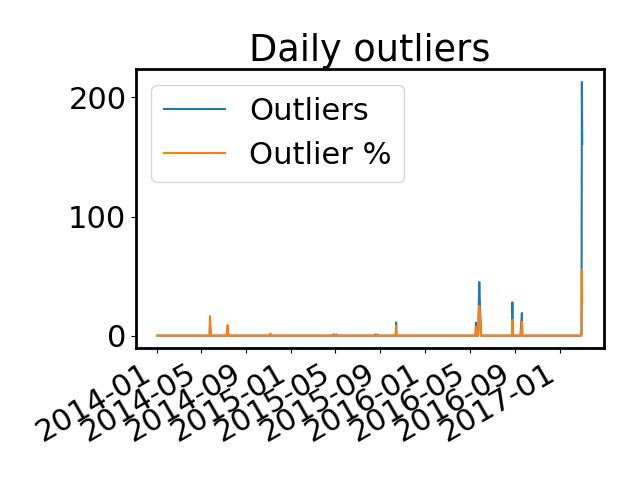
\includegraphics[width = 0.5\textwidth]{report/figures/analysis/plant2_train_long/svm_daily_outliers.png}
    %         \caption{Outlier statistics for svm}
    %         \label{fig:svm_outliers_stats}
    %     \end{figure}
        
        
    
    % \clearpage
    % \subsection{Anomaly detection 3, artificial error}
    %     The anomaly detectors trained on plant 2 are tested on the artificial error created on data from plant 2 not used for training. 
    %     \begin{figure}
    %         \centering
    %         \includegraphics[width=\textwidth]{report/figures/analysis/plant2_train_4months/plant2_artificial_anomaly_datetime.png}
    %         \caption{Anomaly score for the detectors trained on the normal data from plant 2, tested on artificial error data. The red line marks the $1\%$ most extreme scores.}
    %         \label{fig:plant2_arti_anomaly_score}
    %     \end{figure}
        
    %     As seen in figure \ref{fig:plant2_arti_anomaly_score} the detectors clearly detect the artificial error. The error is as explained above constructed to increase its effect gradually, and all three detectors can detect this pattern. It also looks similar to the pattern seen for the production data from plant 1. This further strengthens the claim that the error reported in March 2017, could be traced in the needle operation from early fall 2016. The artificial error is added to production data for plant $2$ from $2015$. This means that it is not seen by the detectors since they are trained from production data from $2016$.  
        
        
        
        
    % not possible to use any time-series forecasting since the data is not sampled at even frequencies. hence using a regression model and estimating an anomaly based on differences from the sampled and predicted data becomes invalid. 
    
    % bruke kde men det vil antagelig ikkje gje gode resultat sidan samplinga mi er dårlig, og eg ikkje har nok data spredd godt nok utover tilstandsrommet. 

% \section{Unsupervised dimensionallity reduction}\label{sec:dim_reduc}

%     \subsection{PCA}\label{subsec:PCA}


%     \subsection{Kernel PCA}\label{subsec:K_PCA}
    


% \section{Pelton needles}\label{sub:pelton_needles}
%     As mentioned, there was data available from three different power plants with Pelton turbines. One of the plants had recorded several issues with the needle control and was used as a case to test early detection of problems with the needle operation. 
    
    
%     \begin{figure}
%         \centering
%         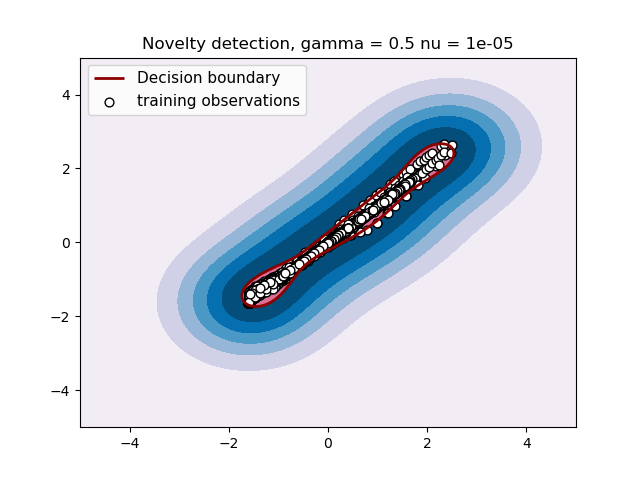
\includegraphics[scale=0.8]{report/figures/analysis/hjartdola/hjar_n2_4_novelty_05_1e-5_train.png}
%         \caption{OCSVM trained on data after overhaul in Mars 2017}
%         \label{fig:my_label}
%     \end{figure}


    
%     \begin{figure}
%         \centering
%         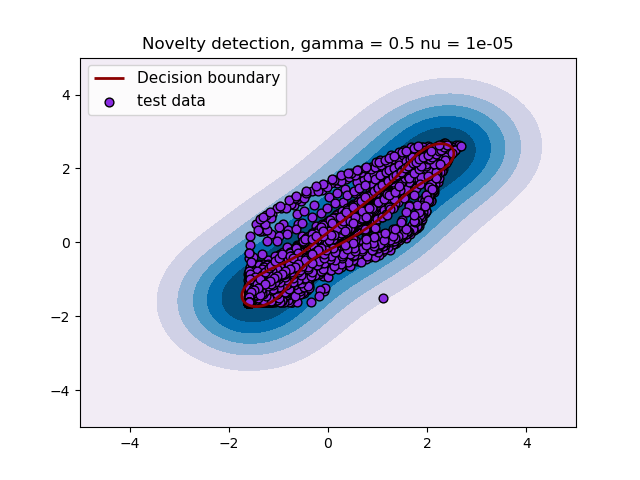
\includegraphics[scale=0.8]{report/figures/analysis/hjartdola/hjar_n2_4_novelty_05_1e-5_test.png}
%         \caption{All process data from before the overhaul}
%         \label{fig:my_label}
%     \end{figure}



